%% First full draft, 2026-10-01.
%% NOTE: the SIAM class (siamart220329.cls) is not installed on this machine, so this draft
%% uses the standard article class. Swap in the SIAM template (\documentclass{siamart220329},
%% \headers, \author with \thanks, etc.) before submission.
%% Every number below comes from the git log, docs/WORKLOG.md, results/families/nrho_id53/*,
%% results/families/nrho_id97/*, results/families/elliptic_members_scan.txt, or
%% figures/family_id{53,97}/id{53,97}_table.csv. Items marked TODO need input from the author.
%% Revised 2026-10-01: Results rewritten around the NRHO Id 53 family.
%% Revised 2026-10-05: new Sec. on the limits of the families and their breakdown
%% (results/families/stability_edge_scan.txt, figures/breakdown/limits_*.{png,csv}); large-torus
%% runs (Ids 51, 101, 87, Id 37 second slice) and the outward extensions added to the tables
%% (docs/STATUS_2026-10-05.md, results/families/nrho_id*/OUTWARD_EXTENSIONS.md, git log).

\documentclass[11pt]{article}

\usepackage[margin=1in]{geometry}
\usepackage{amsmath,amssymb,amsthm}
\usepackage{graphicx}
\usepackage{booktabs}
\usepackage[hidelinks]{hyperref}
\usepackage[capitalise]{cleveref}

\graphicspath{{figures/}}

\newtheorem{remark}{Remark}
\newcommand{\T}{\mathbb{T}}
\newcommand{\R}{\mathbb{R}}
\newcommand{\Z}{\mathbb{Z}}
\newcommand{\avg}[1]{\langle #1 \rangle}
\newcommand{\todo}[1]{\textbf{TODO: #1}}
\DeclareMathOperator{\err}{err}

\title{Lagrangian invariant tori around near-rectilinear halo orbits\\
of the Saturn--Enceladus system by the parameterization method}
\author{Jared Blanchard\thanks{\todo{affiliation}. Email: \todo{contact email}.}}
\date{\todo{date / conference}}

\begin{document}
\maketitle

\begin{abstract}
Near-rectilinear halo orbits (NRHOs) of the Saturn--Enceladus circular restricted three-body
problem (CR3BP) are candidate orbits for an Enceladus orbiter. Around the nearly stable members
of this family lie two-parameter families of quasi-periodic orbits, which offer design freedom
beyond the periodic orbit itself. We compute these quasi-periodic orbits as Lagrangian invariant
2-tori of a four-dimensional Poincar\'e map at fixed energy, using the KAM-inspired
parameterization method of Haro and Luque. A quasi-Newton step solves the invariance equation in
an approximately symplectic frame by means of cohomological equations, at a cost of
$O(N\log N)$ operations plus $N$ map evaluations for $N$ grid points. Making the method work for
tori a few kilometres across, sitting at a distance of order one from the origin, required a set
of practical ingredients: torus-adapted symplectically normalized coordinates rebuilt along the
family, scale-free thresholds, an invariance error measured in the sup norm in physical units,
low-pass filtering, stall detection at the noise floor of the map, and grid refinement. We
verify the solver on an integrable twist map with exact tori, where it converges quadratically,
and on the CR3BP, where one Newton step reduces the invariance error of an orbit-fitted torus
from $1.12\times10^{-10}$ to $5.37\times10^{-13}$ length units (LU). A scan of the elliptic NRHO members shows that their perilune altitude above
Enceladus falls from $28$~km to below the surface as the orbits approach the moon, so the choice
of member matters. Continuation in the rotation vector produces a family of 109 tori around NRHO
Id~53 (perilune $17.1$~km), with radii from $1.35$ to $14.7$~km on the section, median invariance
errors of $4.5\times10^{-13}$ and $1.9\times10^{-12}$~LU on its two branches and a maximum of
$9.9\times10^{-12}$~LU (about $2$~mm); the quasi-periodic orbits of its largest torus stay at
least $8.9$~km above the surface; an extension with a relaxed tolerance floor takes it to
$15.4$~km. Around NRHO Id~97, numerically just as well behaved but with a
perilune of only $4.2$~km, the larger tori of a 141-torus family ($0.67$ to $9.4$~km) impact
Enceladus. Families around six more members, some started in a different mix of the two
elliptic modes, give the largest torus computed, $20.0$~km around NRHO Id~51. We also determine
how large the tori can get. Orbit sweeps show that the regular region around each NRHO reaches at
most about $16$ to $21$~km on the section. Near its edge the frequency drift of orbits crosses the
regularity threshold, and the number of Fourier modes the tori need grows rapidly and
anisotropically. The families therefore end close to the breakdown of the tori, not only at a
numerical limit.
\end{abstract}

%% ============================================================================
\section{Introduction}\label{sec:intro}

Enceladus is a high-priority target for future exploration because of the plumes that vent
material from its subsurface ocean, and orbiter concepts have been studied for it
\cite{cable2021enceladus}. Its small mass parameter in the Saturn system makes the design of
orbits around it a genuinely three-body problem, and Saturnian-moon orbits have been explored in
the CR3BP \cite{davis2018saturnian}. Near-rectilinear halo orbits (NRHOs), the members of the
$L_1$/$L_2$ halo families that pass close to the smaller primary, have been studied extensively in
the Earth--Moon system \cite{zimovan2017nrho,zimovanspreen2020,whitley2016options}, where some of
them are nearly stable. In the Saturn--Enceladus system the corresponding NRHOs are short-period
orbits (about $11.6$~h for NRHO Id~97 below) with a close passage over Enceladus, a few to a few
tens of kilometres above its surface.

Around a linearly stable periodic orbit, KAM theory predicts a Cantor family of invariant tori
carrying quasi-periodic orbits (QPOs) \cite{kolmogorov1954,arnold1963proof,moser1962}. QPOs
enlarge the design space around a baseline periodic orbit, and they have been computed in
astrodynamics and dynamical systems by several methods: semi-analytic normal-form and
Fourier-based approaches \cite{jorba1999normal,gomezmondelo2001,jorba2001numerical},
collocation-type methods for invariant circles of stroboscopic or Poincar\'e maps
\cite{olikara2016computation,baresi2018qpo,mccarthy2021qpo}, and pseudo-arclength continuation of
tori \cite{schilder2005continuation}. The parameterization method
\cite{gonzalez2005kam,haro2006parameterization,haro2016book} takes a different route: it solves
the invariance equation of the torus by a Newton-like method that exploits the geometry of the
problem (symplecticity and the Lagrangian character of the torus). In the KAM setting the
resulting quasi-Newton step reduces to cohomological equations with constant coefficients, which
are solved diagonally in Fourier space
\cite{haroluque2016ch4,figueras2017rigorous}. The method has an a-posteriori theory behind it: an
approximately invariant torus that satisfies explicit non-degeneracy and non-resonance conditions
is close to a true invariant torus \cite{gonzalez2005kam,figueras2017rigorous}. It has been
adapted to flows and to partially hyperbolic tori
\cite{haromondelo2021flow,haroluque2019partially,fernandezmora2024siads,fernandezmora2026convergence},
and to whiskered tori in periodically perturbed restricted three-body problems
\cite{kumar2022whiskered}.

This paper applies the parameterization method of Haro and Luque
\cite{haroluque2016ch4,figueras2017rigorous} to Lagrangian invariant tori around NRHOs of the
Saturn--Enceladus CR3BP. We work with the Poincar\'e map on the section $q_3=0$ at fixed energy,
a four-dimensional symplectic map whose Lagrangian 2-tori correspond to quasi-periodic orbits
with three frequencies (two frequencies and the return time). The contributions are:
\begin{itemize}
\item A computational framework for these tori, built on the parameterization-method KAM code of
  Haro and Luque and on the CR3BP and Poincar\'e-section library of Haro and Mondelo, and adapted
  to Cartesian tori around an elliptic fixed point of a Poincar\'e map (\cref{sec:model,sec:method}).
\item A set of practical ingredients that this problem needed and that we found essential for
  convergence: tori are small (of order $10^{-5}$~LU) and far from the origin, which breaks
  absolute thresholds, error measures and fixed frames that are harmless for maps on
  $\T^d\times\R^d$ (\cref{sec:practical,sec:lessons}).
\item A verification suite: Jacobian and symplecticity checks, an integrable twist map with exact
  tori, and a free-frequency test (\cref{sec:verification}).
\item A scan of the elliptic NRHO members by perilune altitude and distance to low-order
  resonances, used to select the members to compute (\cref{sec:scan}).
\item A family of 109 tori around NRHO Id~53, with radii from $1.35$ to $14.7$~km and invariance
  errors of $10^{-13}$ to $10^{-11}$~LU, whose quasi-periodic orbits stay at least $8.9$~km above
  Enceladus; and, for contrast, a family of 141 tori around the lower NRHO Id~97, whose larger
  tori impact Enceladus (\cref{sec:results}). Families around Ids~23, 37 and 85, and large-torus
  runs around Ids~51, 87 and 101 with start tori in other mode mixes, the largest torus being
  $20.0$~km around Id~51 (\cref{sec:summary}).
\item An analysis of the limits of the families (\cref{sec:limits}): the extent of the regular
  region around each elliptic NRHO, measured by orbit sweeps, and two signatures of the approach
  to breakdown of the tori near its edge, the frequency drift of orbits and the growth of the
  Fourier modes the tori need. Tori whose quasi-periodic orbits intersect the surface are kept and
  marked, since the point-mass model does not see Enceladus.
\end{itemize}
\todo{Check whether QPOs around Saturn--Enceladus NRHOs have been computed before, and adjust
the wording of the contribution list accordingly.}

%% ============================================================================
\section{Model}\label{sec:model}

\subsection{The CR3BP in Hamiltonian form}
We use the CR3BP in the rotating frame with the conventions of the Barcelona RTBP library
(normalized units, the large primary at $(\mu,0,0)$ and the small one at $(\mu-1,0,0)$). With
positions $q=(q_1,q_2,q_3)$ and momenta $p=(p_1,p_2,p_3)$ the Hamiltonian is
\begin{equation}\label{eq:ham}
H(q,p) = \tfrac12\left(p_1^2+p_2^2+p_3^2\right) + q_2 p_1 - q_1 p_2 - \frac{1-\mu}{r_1} - \frac{\mu}{r_2},
\end{equation}
with $r_1 = |q-(\mu,0,0)|$ and $r_2 = |q-(\mu-1,0,0)|$ \cite{szebehely1967,koon2011}. For
Saturn--Enceladus we use
\[
\mu = 1.901109735892602\times10^{-7}, \qquad 1~\mathrm{LU} = 238042~\mathrm{km}
\]
(the length unit is the Saturn--Enceladus distance). The equations of motion and their
first variational equations are integrated with a Runge--Kutta--Fehlberg 7(8) method
\cite{fehlberg1968rk78} with local tolerance $4\times10^{-14}$.
\todo{Confirm that rk78vp.c is the Fehlberg 7(8) pair, and give the source of
\nolinkurl{data/initial_conditions/NRHO_L2.csv} (\nolinkurl{docs/PROVENANCE.md} lists it as open).}

\subsection{Poincar\'e section at fixed energy}
We fix the energy $H=h$ and take the section $\Sigma = \{q_3 = 0,\ p_3>0,\ H=h\}$. On $\Sigma$ we
use the coordinates $z=(q_1,q_2,p_1,p_2)$ and recover $p_3>0$ from \eqref{eq:ham}:
\begin{equation}\label{eq:p3}
p_3(z)^2 = 2\left(h - q_2 p_1 + q_1 p_2 + \frac{1-\mu}{r_1} + \frac{\mu}{r_2}\right) - p_1^2 - p_2^2 .
\end{equation}
Let $\nu(z) = (q_1,q_2,0,p_1,p_2,p_3(z))$ lift a point of the section to $\R^6$, and let $\pi$ be
the projection back to $(q_1,q_2,p_1,p_2)$. The reduced map is $F = \pi\circ P\circ\nu$, where
$P$ is the first-return map of the flow to $\{q_3=0\}$ in the direction of increasing $q_3$. Since
$\Sigma$ lies in an energy level, $F$ is symplectic for the standard form
$\Omega = \left(\begin{smallmatrix} 0 & -I_2\\ I_2 & 0\end{smallmatrix}\right)$ in $z$ \cite[Remark~2.4.5, p.~8]{haromondelo2021flow}; on a simply connected domain it
is also exact symplectic.

\subsection{Differential of the map}
Let $\Phi$ be the state transition matrix from $\nu(z)$ to the return point $x_\tau = P(\nu(z))$,
$f$ the vector field and $g(x)=q_3$ the section function. The differential of the return map is
\begin{equation}\label{eq:DP}
DP = \Phi + f(x_\tau)\, D\tau^{\!\top}, \qquad
D\tau^{\!\top} = -\frac{\nabla g^{\top}\Phi}{\nabla g\cdot f(x_\tau)},
\end{equation}
\cite[Sec.~7, eqs.~(40) and (42), pp.~17--18]{wilczak2007lohner}, and
$DF(z) = \pi\, DP\, D\nu(z)$, where $D\nu$ contains the gradient of $p_3$ from \eqref{eq:p3}
(by the chain rule, $\nabla p_3 = \nabla(p_3^2)/(2p_3)$). The return to the section is refined by
Newton's method on $q_3$ to a tolerance of $10^{-14}$.

\subsection{NRHOs as fixed points}
A periodic orbit that crosses $\Sigma$ once per period is a fixed point $z^*$ of $F$. We compute it
by Newton's method on $F(z)-z=0$ from the initial conditions of our NRHO table. The eigenvalues of
$DF(z^*)$ come in pairs $\lambda,1/\lambda$ (and conjugates); for the nearly stable NRHOs used
here both pairs lie on the unit circle, $\lambda_j = e^{\pm 2\pi i \rho_j}$, and we call
$\rho = (\rho_1,\rho_2)$ the linear rotation numbers of the NRHO. Invariant tori of $F$ around
$z^*$ are Cartesian: they are graphs over neither the angles nor the positions, and the
parameterization $K:\T^2\to\R^4$ is fully periodic (no angle lift).

%% ============================================================================
\section{Method}\label{sec:method}

\subsection{Invariance equation}
We look for $K:\T^2\to\R^4$ and $\omega\in\R^2$ such that
\begin{equation}\label{eq:inv}
E(\theta) := F(K(\theta)) - K(\theta+\omega) = 0
\end{equation}
\cite[Sec.~2.1, eq.~(4), p.~5]{figueras2017rigorous}, \cite{fontich2009kam}. With $\omega$
irrational, an invariant torus is Lagrangian, $DK^\top \Omega\, DK = 0$
\cite{figueras2017rigorous}. We represent $K$ on an $n_1\times n_2$ grid of $\T^2$ and by its
discrete Fourier transform, and we measure the error by the sup norm over the grid in physical
coordinates,
\begin{equation}\label{eq:err}
\err(K) = \max_{j}\ \| E(\theta_j) \|_\infty ,
\end{equation}
as in \cite[Alg.~3.6.1, p.~29]{haromondelo2021flow} (see \cref{sec:practical}).

\subsection{Symplectic frame, torsion and the quasi-Newton step}
We follow Figueras, Haro and Luque \cite{figueras2017rigorous}; see also
\cite{haroluque2016ch4,haro2016book}. Let $L(\theta)=DK(\theta)$. Given a positive definite
metric $G$, the normal frame
\begin{equation}\label{eq:frame}
N = L A - \Omega^{-1} G L B, \qquad B = \left(L^\top G L\right)^{-1}, \qquad
A = \tfrac12\, B^\top L^\top G\, \Omega^{-1} G\, L B ,
\end{equation}
(\cite[eq.~(32), p.~14]{haromondelo2021flow}, written as in our code) makes
$P(\theta)=(L(\theta)\ N(\theta))$ symplectic up to $O(E)$. In this frame the linearized dynamics
is approximately block triangular,
$P(\theta+\omega)^{-1} DF(K(\theta)) P(\theta) \approx
\left(\begin{smallmatrix} I & T(\theta)\\ 0 & I\end{smallmatrix}\right)$, with the torsion
\begin{equation}\label{eq:torsion}
T(\theta) = N(\theta+\omega)^\top\, \Omega\, DF(K(\theta))\, N(\theta)
\end{equation}
\cite[eqs.~(8)--(13), p.~6]{figueras2017rigorous}. Writing the correction as
$\Delta K = P\xi$ in the linearized equation
\cite[eq.~(25), p.~9]{figueras2017rigorous}
\begin{equation}\label{eq:lin}
DF(K(\theta))\,\Delta K(\theta) - \Delta K(\theta+\omega) = -E(\theta)
\end{equation}
and dropping $O(E)$ terms gives, with
$\eta_L = -N(\theta+\omega)^\top\Omega E$ and $\eta_N = L(\theta+\omega)^\top\Omega E$, a
triangular system of cohomological equations. Its solution is
\cite[Lemma~2.9, eqs.~(32)--(34), p.~10]{figueras2017rigorous}
\begin{equation}\label{eq:xi}
\xi_N = \mathcal{R}(\eta_N) + \xi_N^0, \qquad
\xi_L = \mathcal{R}(\eta_L - T\xi_N) + \xi_L^0, \qquad
\xi_N^0 = \avg{T}^{-1}\avg{\eta_L - T\mathcal{R}(\eta_N)},
\end{equation}
where $\mathcal{R}v$ is the zero-average solution of $u(\theta)-u(\theta+\omega) = v(\theta)-\avg{v}$,
\begin{equation}\label{eq:cohom}
\widehat{u}_k = \frac{\widehat{v}_k}{1-e^{2\pi i k\cdot\omega}}, \qquad k\neq 0
\end{equation}
\cite[eq.~(20), p.~7]{figueras2017rigorous}, and $\xi_L^0$ (a phase) is set to zero. The
non-degeneracy (twist) condition is $\det\avg{T}\neq 0$ \cite[Lemma~2.9, p.~10]{figueras2017rigorous};
for an invariant Lagrangian torus $\avg{T}$ is symmetric, which is a useful diagnostic. The step
converges quadratically \cite[Lemma~2.8, eq.~(31), p.~10]{figueras2017rigorous}. Every operation
is either pointwise on the grid or diagonal in Fourier space, so a step costs $O(N\log N)$
operations with $N=n_1n_2$, plus $N$ evaluations of $F$ and $DF$. In the CR3BP the map
evaluations dominate.

A frequency-adjusting variant fixes $\xi_N^0=0$ and corrects $\omega$ instead, with
$\Delta\omega = -\avg{\eta_L - T\mathcal{R}(\eta_N)}$, the solvability condition of the tangent
row; this is in the spirit of \cite[Sec.~6.1, eqs.~(6.1)--(6.6), p.~45]{haroluque2019partially}
and needs no inverse of $\avg{T}$. We use it only as a test (\cref{sec:verification}); the family
is computed at fixed $\omega$.

\subsection{Practical ingredients}\label{sec:practical}
The tori of interest have radii of $10^{-5}$ to $10^{-4}$~LU, sit at $|z|\approx 1$, and are very
eccentric in the original coordinates (the entries of $DF$ are of order 27). The following
ingredients were needed for the quasi-Newton step to converge on them. \Cref{sec:lessons}
discusses why.

\paragraph{Torus-adapted symplectic coordinates.} We solve for $K$ in local coordinates
$z = z_c + M\zeta$, where $z_c$ is the average of the torus and the columns of $M$ are its
first-harmonic axes, $a_j = 2\,\mathrm{Re}\,\widehat{K}_{e_j}$ and
$b_j = -2\,\mathrm{Im}\,\widehat{K}_{e_j}$. Each pair is normalized so that
$a_j^\top\Omega b_j = -1$, and then all columns are rescaled so that the torus is close to a
product of circles of radius one in $\zeta$. The change is affine, so the map and its Jacobian
become $\tilde F(\zeta) = M^{-1}(F(z_c+M\zeta)-z_c)$ and $D\tilde F = M^{-1}DF\,M$, and the
symplectic form becomes the constant $M^\top\Omega M$ divided by the square of the rescaling
factor, close to the standard form. In these coordinates we use the Euclidean metric $G=I$ in
\eqref{eq:frame}. This is the familiar idea of working in coordinates adapted to the linearization
(a symplectic Floquet-like normalization), here taken from the torus itself. Because the torus
changes shape and size along the family, the coordinates are rebuilt from every accepted torus
during continuation.

\paragraph{Scale-free thresholds.} Coefficients of the right-hand side of \eqref{eq:cohom} are
skipped only if they are small relative to the largest one, not below an absolute threshold.

\paragraph{Nyquist modes.} On an even grid the Nyquist coefficient has no conjugate partner.
Differentiation, translation by $\omega$, and \eqref{eq:cohom} then produce a non-Hermitian
spectrum, i.e.\ complex values in real space. We set these modes to zero in all three operations
and when the grid is refined, and we drop the (round-off level) imaginary part of $K$ after each
step.

\paragraph{Shifted normal frame.} The frame at $\theta+\omega$ needed in $\eta_L$ and
\eqref{eq:torsion} is computed by applying \eqref{eq:frame} pointwise to the Fourier-shifted $L$
(and metric and form), not by shifting $N$: the spectrum of $N$, which contains
$(L^\top G L)^{-1}$, decays more slowly than that of $L$.

\paragraph{Error measure.} The error \eqref{eq:err} is the maximum over the grid in physical
coordinates, $E_{\mathrm{phys}} = M E$. The $\ell^1$ norm of all Fourier coefficients, used in an
earlier version of the code, sums the noise of every coefficient and grows with the grid size.

\paragraph{Low-pass filter.} After each step we set to zero all Fourier coefficients with
$|k_j|\ge n_j/4$ in some direction. Haro and Mondelo report ``divergence after apparent
convergence'' even with tails of the order of machine epsilon, and prevent it by zeroing the upper
half of the DFT after each Newton iteration \cite[pp.~27--28]{haromondelo2021flow}; see also
\cite{kumar2022whiskered}. The relative error of the DFT coefficients grows with $|k|$, and the
small divisors in \eqref{eq:cohom} amplify it.

\paragraph{Stall detection and the map-noise floor.} The error can only be reduced to the
accuracy of the map evaluation. Beyond that point further steps amplify the noise through the
small divisors and the iteration drifts away. The Newton loop keeps the best torus, stops when a
step fails to reduce the error by at least $10\%$, and accepts the best torus if its error is below
a floor $\epsilon_{\mathrm{floor}}$ (we use $10^{-11}$~LU, about $2.4$~mm); the strict tolerance
is $10^{-12}$~LU.

\paragraph{Grid refinement.} If Newton stalls above $\epsilon_{\mathrm{floor}}$, the torus is
interpolated to a grid twice as fine in each direction (zero padding) and Newton continues, once
per loop. This is step 5 of \cite[Alg.~3.6.1, p.~30]{haromondelo2021flow}: ``if
$\mathrm{err}(T')>\varepsilon_1$, double $N$''. We refine only if the best error is within a
factor $100$ of $\epsilon_{\mathrm{floor}}$; stalls farther above it, which occur when a
continuation predictor has left the basin of convergence, are handled by halving the
continuation step instead. The original branches of the main families were computed with refinement in both directions and
a largest grid of $128\times128$. For the larger tori we refine anisotropically
(\cref{sec:limits-response}): we measure, per angle, the fraction of the error spectrum in the band
$3n_j/16\le|k_j|<n_j/4$ just below the filter cutoff, and double only the angle(s) in which the best
torus has at least $20\%$ of its error spectrum there; otherwise the step is rejected and halved.
After an accepted torus whose error exceeds $0.3\,\epsilon_{\mathrm{floor}}$ we refine in the same
way before the next step (proactive refinement). The grid cap is then $262144$ points (e.g.\
$512\times512$).

\paragraph{Continuation.} We continue tori at fixed energy in the rotation vector
\cite[Sec.~3.5, Alg.~3.5.4]{haromondelo2021flow}, along a straight line
$\omega(\varepsilon) = \omega_s + \varepsilon\,\Delta\omega$. The predictor is the secant through
the last two tori (Haro and Mondelo use a tangent predictor). The step control follows
\cite[Alg.~3.6.1, pp.~29--30]{haromondelo2021flow}: halve the step on failure and, after a success,
multiply it by $n_{\mathrm{des}}/n_{\mathrm{it}}$ with $n_{\mathrm{des}}=4$ desired iterations
(clamped to $[0.5,2]$); stop when the step falls below $10^{-3}$ of the initial one or $\varepsilon$
reaches a prescribed limit. Since Lagrangian tori of a 4D map at fixed energy form a two-parameter
(Cantor) family indexed by $\omega$, a line in $\omega$ selects a one-parameter path through it.

\subsection{Initial guesses}\label{sec:guess}
Initial tori come from orbits of $F$. We start at $z^* + a_1\mathrm{Re}\,V_1 + a_2\mathrm{Re}\,V_2$,
where $V_j$ are the elliptic eigenvectors of $DF(z^*)$ and $(a_1,a_2) = a\,(c_1,c_2)$ with a
\emph{mode mix} $(c_1,c_2)$, $(1,1)$ for the main families, iterate the map, and compute the rotation
numbers of the orbit from its complex eigen-coordinates: a linear fit of the unwrapped angle,
refined by maximizing the Hann-windowed Fourier amplitude as in Laskar's NAFF
\cite{laskar1990chaotic,laskar1993naff}. We then fit the Fourier coefficients of $K$ to the orbit
by least squares, $z_m \approx K(m\rho)$, with $|m_i|\le 10$. The same tools give a frequency map
of the neighborhood of the NRHO, with the drift of the rotation numbers between the two halves of
an orbit as a regularity indicator \cite{laskar1993naff}.

%% ============================================================================
\section{Verification}\label{sec:verification}

\paragraph{Map and Jacobian.} The analytic $DF$ agrees with central finite differences
($h=10^{-7}$) to a relative $5.7\times10^{-7}$, and $DF$ is symplectic for the standard form to
$5\times10^{-10}$. \todo{State exactly which quantity gave $5\times10^{-10}$ (presumably
$\|DF^\top\Omega DF-\Omega\|$) and at which point.} The second difference
$|F(z+hv)-2F(z)+F(z-hv)|/h^2$ at the fixed point of NRHO Id~72 is constant ($2.2\times10^5$) from
$h=10^{-3}$ down to $3\times10^{-9}$, so the map is smooth down to below $10^{-13}$; it also gives
a nonlinearity length scale of $1/(2.2\times10^5)\approx 5\times10^{-6}$~LU, about 1~km. Newton's
method for the fixed point of NRHO Id~72 converges quadratically,
$|F(z)-z| = 3.9\times10^{-7},\ 2.5\times10^{-11},\ 2.7\times10^{-14}$; this orbit is
elliptic-elliptic with $\rho = (0.343616643, 0.173806970)$.

\paragraph{Integrable twist map.} The map that rotates each plane $(q_j,p_j)$ by the angle
$2\pi\big(\rho_j + \sum_k b_{jk} I_k\big)$, $I_k = (q_k^2+p_k^2)/2$, is the time-one map of
$H = 2\pi\rho\cdot I + \pi I^\top b I$. It is symplectic for the same form as the CR3BP map, and its
tori are known exactly: $K_j(\theta) = \sqrt{2I^*_j}\,(\cos 2\pi\theta_j, \sin 2\pi\theta_j)$ with
$\rho + bI^* = \omega$. Like the NRHO tori, they are Cartesian tori around an elliptic fixed point,
so this map exercises the same code path. Starting from the exact torus with a $1\%$ error in the
actions plus a $10^{-4}\cos 2\pi(\theta_1+\theta_2)$ perturbation, on a $32\times32$ grid, the
error decreases quadratically (\cref{tab:twist}). The averaged torsion is symmetric,
$\avg{T} = \left(\begin{smallmatrix}-0.1592 & -0.0478\\ -0.0478 & -0.0796\end{smallmatrix}\right)$.
A frame built from a constant transversal field (the momentum directions) instead of
\eqref{eq:frame} fails on this map ($\avg{T}\sim 10^{26}$): around an elliptic point,
$DK^\top\Omega N_0$ is singular where $\sin 2\pi\theta_j = 0$, violating the transversality
condition \cite[eq.~(7), p.~6]{figueras2017rigorous}.

\begin{table}[t]
\centering
\caption{Quasi-Newton iteration on the integrable twist map, $32\times32$ grid, fixed $\omega$.
Sup-norm error \eqref{eq:err} with the current code; the linearized residual and the frame check
$|L^\top\Omega N + I|$ were measured with an earlier version of the code (Fourier $\ell^1$ norm).}
\label{tab:twist}
\begin{tabular}{cccc}
\toprule
iteration & $\err(K)$ & linearized residual & frame check \\
\midrule
1 & $2.1\times10^{-4}$  & $4.4\times10^{-7}$  & $1.2\times10^{-7}$ \\
2 & $1.3\times10^{-6}$  & $2.3\times10^{-11}$ & $3.7\times10^{-12}$ \\
3 & $7.1\times10^{-11}$ & $1.3\times10^{-15}$ & $4.4\times10^{-13}$ \\
4 & $1.1\times10^{-16}$ & ---                 & --- \\
\bottomrule
\end{tabular}
\end{table}

\paragraph{Free-frequency step.} Starting from a twist-map torus with $1\%$ too much action, the
frequency-adjusting step converges in two steps
($2.2\times10^{-4}\to2.5\times10^{-7}\to5.3\times10^{-13}$) and returns
$\Delta\omega = (1.6000107\times10^{-4},\ 1.2999998\times10^{-4})$, against the exact value
$0.01\,bI^* = (1.6\times10^{-4},\ 1.3\times10^{-4})$.

\paragraph{Independent reference solver.} A dense collocation Newton method (Julia) solves the
full linearized invariance equation on the grid, with two phase conditions, by least squares. It
is a true Newton step at a cost of $O((4N)^3)$. On an orbit-fitted torus around NRHO Id~72
($32\times32$, fixed $\omega$) it reduced the error from $4.8\times10^{-10}$ to
$4.9\times10^{-12}$, which confirmed that the map, its Jacobian and the formulation are mutually
consistent at a time when the quasi-Newton solver still diverged.

%% ============================================================================
\section{Results}\label{sec:results}

\subsection{First targets: NRHO Id~72 and Id~97}\label{sec:choice}
Our first target, NRHO Id~72 of our data set (period $0.4895$~days), is elliptic-elliptic but
close to a $1{:}2$ resonance: $\rho_1-2\rho_2 = -0.0040$ at the fixed point. The frequency map of
its neighborhood shows that orbits with amplitude $a_1\gtrsim2\times10^{-5}$~LU along the first
eigendirection lock to the $1{:}2$ resonance ($\rho_1-2\rho_2=0$ to five digits), orbits with
$a_1\gtrsim 8\times10^{-5}$~LU (and small $a_2$) are chaotic or escape (frequency drift
$10^{-3}$ to $10^{-1}$), and regular orbits (drift $\sim10^{-7}$) occupy only a thin region,
$a_1\lesssim5\times10^{-6}$~LU, $a_2\in[2,8]\times10^{-5}$~LU; the first torus we tried,
$a=(10^{-5},10^{-5})$~LU, sits at the edge of the resonance zone. We therefore moved to NRHO Id~97 (period $2.21528$~TU $=0.48493$~days, stability
index $1.0000000000197$ in our table), whose linear rotation numbers
$\rho^{\mathrm{lin}} = (0.3539576, 0.1943036)$ give $\rho_1-2\rho_2 = -0.0347$, ten times
farther from the $1{:}2$ resonance. Its fixed point on $\Sigma$ is
$z^* = (-1.000283097, -0.001895716, -0.000925503, -1.007691126)$ at energy
$h = -1.50001746408344$ (Jacobi constant $3.00003492816688$); it lies about $456$~km from the center
of Enceladus. Numerically, Id~97 is well conditioned, and the method was developed and verified
on it (\cref{sec:newton,sec:id97}). Physically it is a poor choice: integrating the NRHO in the
full flow (Julia, Vern9, tolerance $10^{-13}$), its perilune is $256.3$~km from the center of
Enceladus, only $4.2$~km above the $252.1$~km mean radius. This led us to scan the whole family.
\todo{Add a frequency-map figure (Id~72 or Id~53).}

\subsection{Selecting NRHO members: perilune altitude and resonances}\label{sec:scan}
For every elliptic-elliptic member of the $L_2$ NRHO table with Id~$\le 111$ (odd Ids) we computed
the period, the perilune altitude above the $252.1$~km mean radius of Enceladus, the linear
rotation numbers, and the nearest resonance $k\cdot\rho^{\mathrm{lin}} = n$ with $|k|_1\le 6$,
together with its distance $|k\cdot\rho^{\mathrm{lin}} - n|$. \Cref{tab:scan} shows a selection.
Two trends constrain the choice. First, the perilune altitude falls monotonically with Id, from
$28.1$~km (Id~15) to $0.2$~km (Id~111); members with Id~$\ge 113$ pass below the surface. Second,
the resonance distance does not vary monotonically: some members sit almost on a low-order
resonance (Id~15 at $10^{-4}$ from $k=(-2,-4)$, Id~59 at $6\times10^{-4}$ from $k=(-2,-2)$, Id~71
and Id~109 at a few $10^{-3}$), while others are separated from the nearest one by $10^{-2}$ or
more (Id~53 at $0.017$, Id~85 and Id~97 at $0.022$ and $0.027$). We therefore chose members that
span the perilune altitudes and avoid near resonances: Ids~23, 37, 53, 85 and 97. Id~53 has a
perilune of $17.1$~km, the largest resonance distance among the members above $10$~km, and a
frequency map that is regular (drift $\sim5\times10^{-10}$) up to amplitudes
$(8\times10^{-5},8\times10^{-5})$~LU; it is our main example.

\begin{table}[t]
\centering
\caption{Representative elliptic members of the NRHO table: period $T$, perilune altitude above
the mean radius of Enceladus, linear rotation numbers, and the nearest resonance with $|k|_1\le6$
and its distance $|k\cdot\rho^{\mathrm{lin}}-n|$. Source:
\nolinkurl{results/families/elliptic_members_scan.txt}.}
\label{tab:scan}
\small
\begin{tabular}{rcrccr}
\toprule
Id & $T$ (TU) & perilune alt.\ (km) & $\rho^{\mathrm{lin}}$ & nearest $k$ & distance \\
\midrule
15  & 2.2824 & 28.1 & $(0.336354, 0.081847)$ & $(-2,-4)$ & 0.0001 \\
23  & 2.2760 & 25.8 & $(0.336377, 0.101653)$ & $(-3,0)$  & 0.0091 \\
37  & 2.2648 & 21.8 & $(0.337056, 0.128252)$ & $(-3,0)$  & 0.0112 \\
53  & 2.2516 & 17.1 & $(0.339096, 0.152183)$ & $(-3,0)$  & 0.0173 \\
59  & 2.2468 & 15.4 & $(0.340223, 0.159501)$ & $(-2,-2)$ & 0.0006 \\
71  & 2.2368 & 11.8 & $(0.343322, 0.172841)$ & $(-1,2)$  & 0.0024 \\
85  & 2.2253 &  7.8 & $(0.348321, 0.185508)$ & $(-4,2)$  & 0.0223 \\
97  & 2.2153 &  4.2 & $(0.353958, 0.194304)$ & $(-4,2)$  & 0.0272 \\
109 & 2.2053 &  0.7 & $(0.360906, 0.201352)$ & $(-5,-1)$ & 0.0059 \\
\bottomrule
\end{tabular}
\end{table}

\subsection{Newton convergence on the CR3BP}\label{sec:newton}
For NRHO Id~97 the start torus is orbit-fitted (\cref{sec:guess}) with amplitudes
$(4\times10^{-5},4\times10^{-5})$~LU,
on a $32\times32$ grid, with rotation numbers $\omega_s = (0.35372425999973, 0.19383759358522)$.
\Cref{tab:newton} shows its Newton history and those of the next two continuation steps. The
first step from the orbit fit reduces the error by more than two orders of magnitude, to
$5.37\times10^{-13}$~LU; continuation steps from the secant predictor converge in two steps. The
residual of the linearized equation after the first step is $1.5\times10^{-12}$, about $1\%$ of the
error, and the frame check is $1.6\times10^{-8}$. The averaged torsion in local coordinates is
symmetric to the printed digits,
$\avg{T} = \left(\begin{smallmatrix}-1.337\times10^{-5} & -1.118\times10^{-4}\\
-1.118\times10^{-4} & 3.862\times10^{-5}\end{smallmatrix}\right)$, with
$\det\avg{T} = -1.30\times10^{-8}$, comparable to the square of its largest entry, so the twist
condition is comfortably satisfied. The nearest resonance $k\cdot\omega\in\Z$ with $|k|\le 12$ at the
start torus is $k=(-1,7)$, with $|k\cdot\omega - 1| \approx 3\times10^{-3}$.
For NRHO Id~53 the start torus is built the same way (amplitudes $(4\times10^{-5},4\times10^{-5})$~LU,
$32\times32$, $\omega_s = (0.3393830664659, 0.1526113801869)$), and one Newton step takes its error
from $8.1\times10^{-12}$ to $6.9\times10^{-13}$~LU. The same construction, now automated, accepted
amplitude $4\times10^{-5}$~LU for NRHOs Id~23, 37 and 85, with rotation-number drifts of
$1.1\times10^{-9}$, $2.0\times10^{-9}$ and $4.5\times10^{-10}$.

\begin{table}[t]
\centering
\caption{Newton histories on the CR3BP section map around NRHO Id~97, $32\times32$ grid, fixed
$\omega$: sup-norm invariance error \eqref{eq:err} in LU. The iteration stops when the error is
below the strict tolerance $10^{-12}$~LU. Source: \nolinkurl{results/families/nrho_id97/inward/run.log}.}
\label{tab:newton}
\begin{tabular}{lccc}
\toprule
torus & iteration 1 & iteration 2 & iteration 3 \\
\midrule
start ($\varepsilon=0$, orbit fit)    & $1.119\times10^{-10}$ & $5.370\times10^{-13}$ & \\
$\varepsilon=-0.020$ (predictor)      & $2.450\times10^{-9}$  & $3.345\times10^{-10}$ & $5.561\times10^{-13}$ \\
$\varepsilon=-0.047$ (predictor)      & $3.233\times10^{-9}$  & $6.024\times10^{-10}$ & $6.047\times10^{-13}$ \\
\bottomrule
\end{tabular}
\end{table}

\subsection{A family of tori around NRHO Id~53}\label{sec:id53}
NRHO Id~53 has period $2.2516$~TU and energy $h = -1.50001738952906$; its fixed point on $\Sigma$,
$z^* = (-1.000318177, -0.001977028, -0.000852904, -1.007444102)$, lies about $477$~km from the
center of Enceladus, and its linear rotation numbers are
$\rho^{\mathrm{lin}} = (0.3390958, 0.1521835)$. We continue along
$\omega(\varepsilon) = \omega_s + \varepsilon\Delta\omega$ with
$\Delta\omega = \omega_s - \rho^{\mathrm{lin}} = (2.8729\times10^{-4}, 4.2791\times10^{-4})$, so
again $\varepsilon=-1$ is the NRHO, with tolerance floor $10^{-11}$~LU. The family was computed in
six consecutive runs, three per direction, each restarting from the last torus of the previous one:
\begin{itemize}
\item inward: cumulative $\varepsilon$ from $0$ to $-0.932$ (the detuning reduced to $7\%$),
  68 tori, radius from $5.7$ down to $1.35$~km. The last run stopped when the continuation step fell
  below its minimum, with errors of about $10^{-11}$;
\item outward: cumulative $\varepsilon$ from $0$ to $3.486$, 46 tori, radius from $5.7$ up to
  $14.7$~km, with automatic refinement from $32\times32$ to $64\times64$ and $128\times128$. The last
  run stopped at errors of about $10^{-11}$ on $128\times128$ (\cref{sec:limits}).
\end{itemize}
Of the 114 tori, 35 are on $32\times32$ grids, 14 on $64\times64$ and 65 on $128\times128$; 109 are
distinct, the others being the start torus and the tori at which runs were joined. They cover
$\rho_2\in[0.15221, 0.15410]$ (\cref{fig:freq}) and radii of $1.35$ to $14.7$~km in $(q_1,q_2)$
(\cref{fig:size,fig:section}). The sup error of invariance has median $4.5\times10^{-13}$~LU on the
inward branch and $1.9\times10^{-12}$~LU on the outward branch, and maximum $9.9\times10^{-12}$~LU,
about $2.4$~mm (\cref{fig:error}). As for Id~97 (\cref{sec:id97}), the radius grows like
$\sqrt{\rho_2-\rho^{\mathrm{lin}}_2}$ near the NRHO (\cref{fig:size}), and the error is smallest on
the middle part of the family and rises towards both ends. Three later restarts of the outward
branch from its last torus, with anisotropic refinement and then with a tolerance floor of
$10^{-10}$~LU (about $2.4$~cm), added 35 tori and took the largest radius from $14.74$ to
$15.37$~km, on grids up to $256\times256$; their errors are at most $7.6\times10^{-11}$~LU. Why the
gain is so small is the subject of \cref{sec:limits}. Unless stated otherwise, the figures and
numbers of this section refer to the 109 tori computed with the $10^{-11}$~LU floor.

\begin{figure}[t]
\centering
\begin{minipage}[t]{0.49\textwidth}
\centering
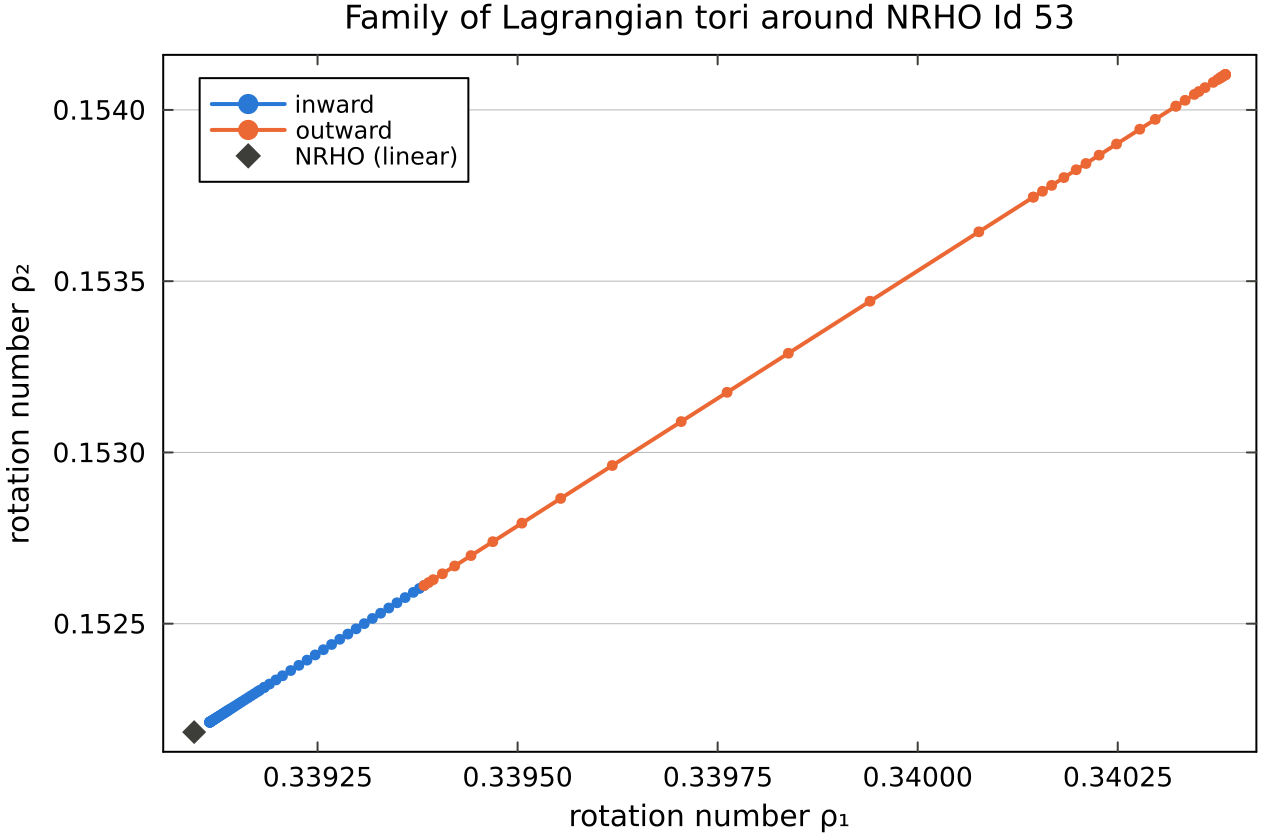
\includegraphics[width=\textwidth]{id53_frequencies.png}
\caption{The family of Lagrangian tori around NRHO Id~53 in rotation-number space. Each marker is
a converged torus; the diamond is the pair of linear rotation numbers of the NRHO.}
\label{fig:freq}
\end{minipage}\hfill
\begin{minipage}[t]{0.49\textwidth}
\centering
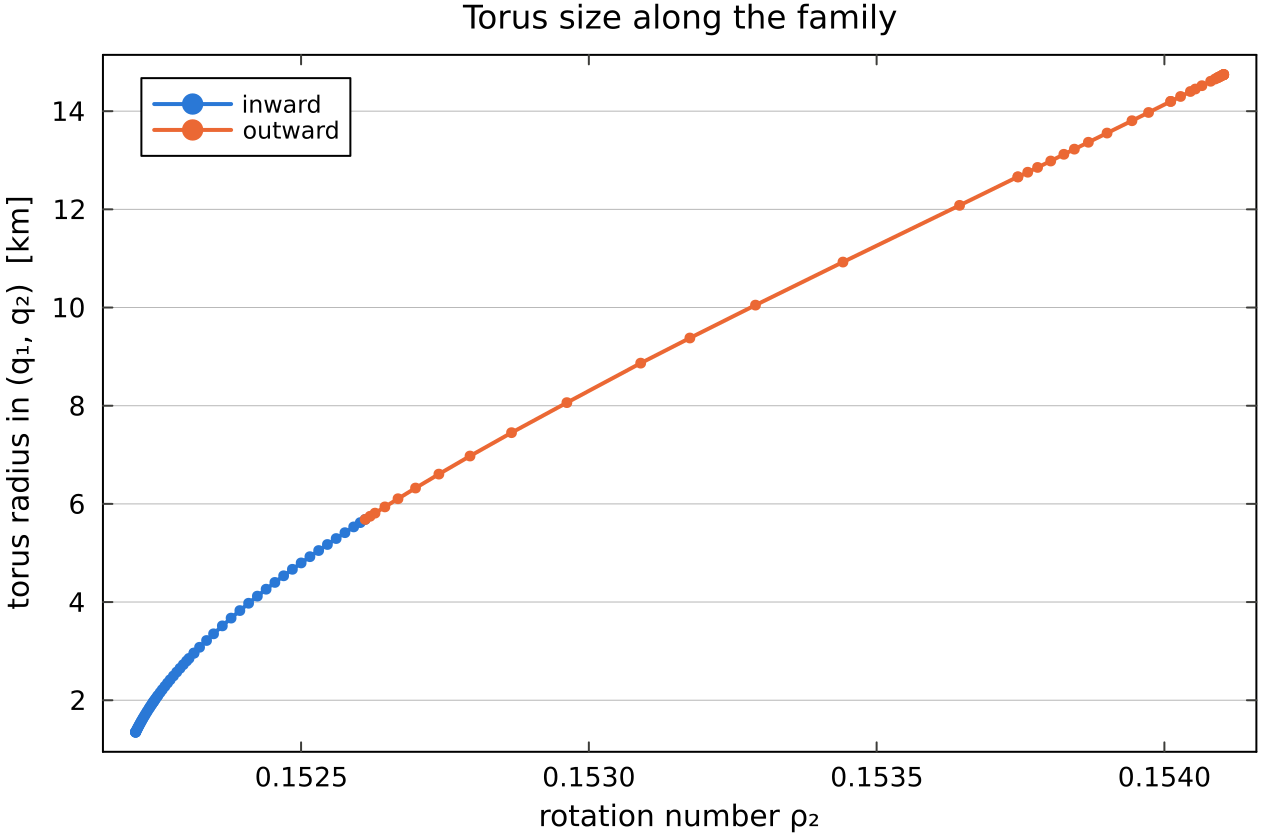
\includegraphics[width=\textwidth]{id53_size.png}
\caption{Torus radius in $(q_1,q_2)$ on the section (maximum distance from the center of the
torus, km) along the Id~53 family.}
\label{fig:size}
\end{minipage}
\end{figure}

\begin{figure}[t]
\centering
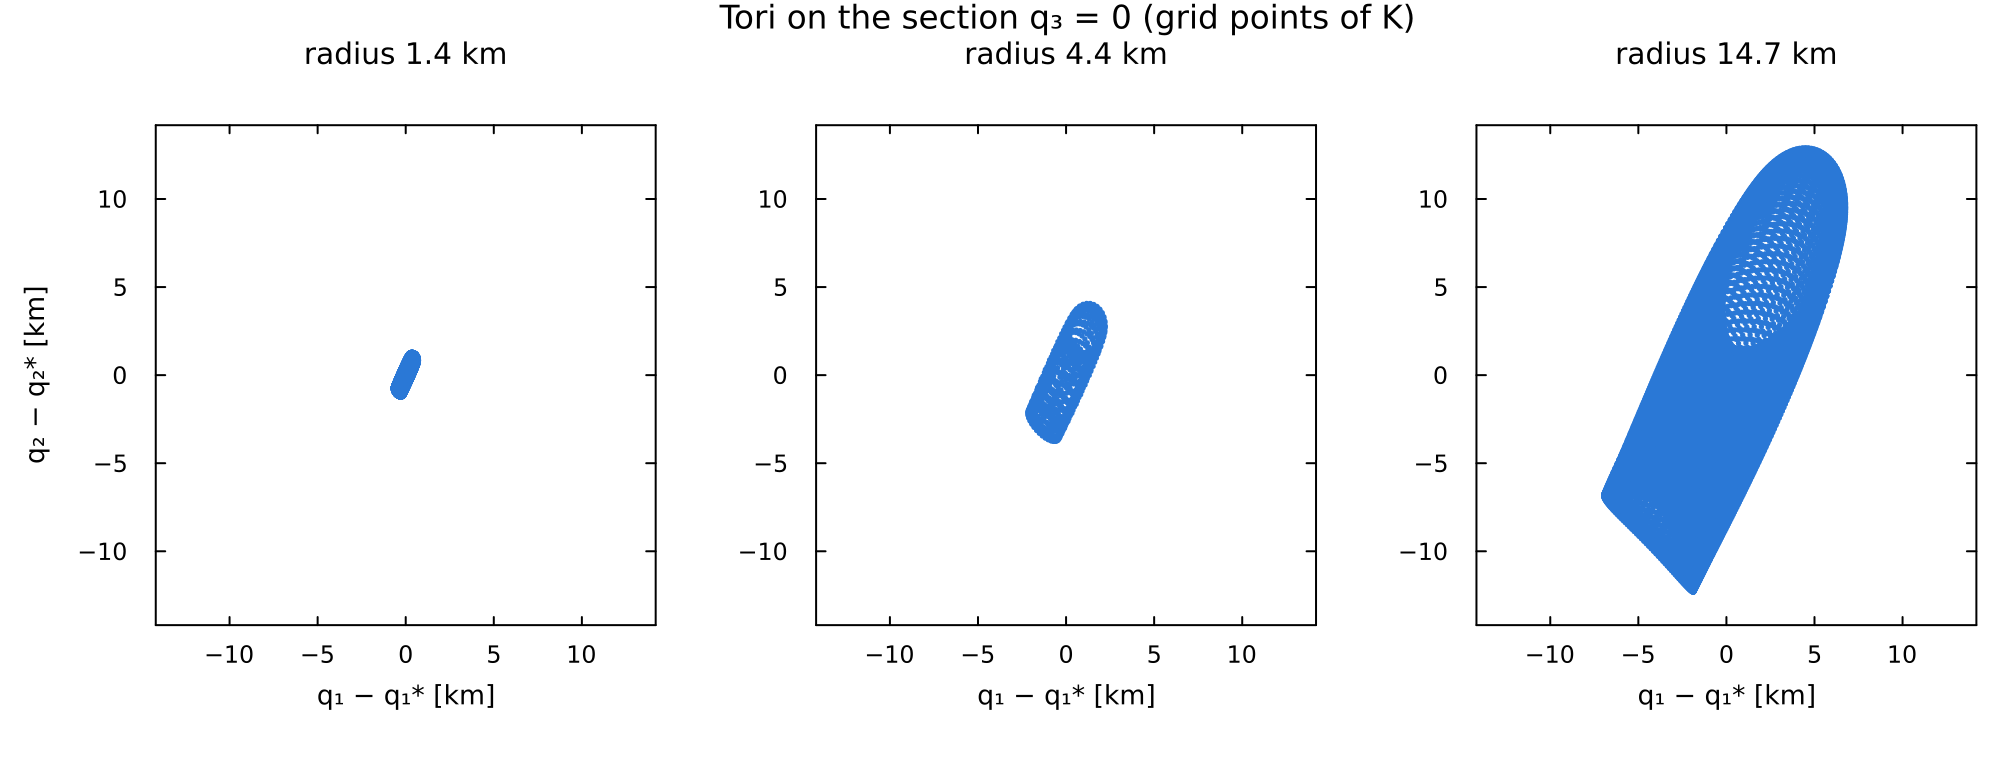
\includegraphics[width=\textwidth]{id53_section.png}
\caption{The smallest, a middle and the largest torus of the Id~53 family on the section $q_3=0$,
projected to $(q_1,q_2)$ relative to the fixed point $z^*$, on a common scale. Each dot is a grid
point of $K$.}
\label{fig:section}
\end{figure}

\begin{figure}[t]
\centering
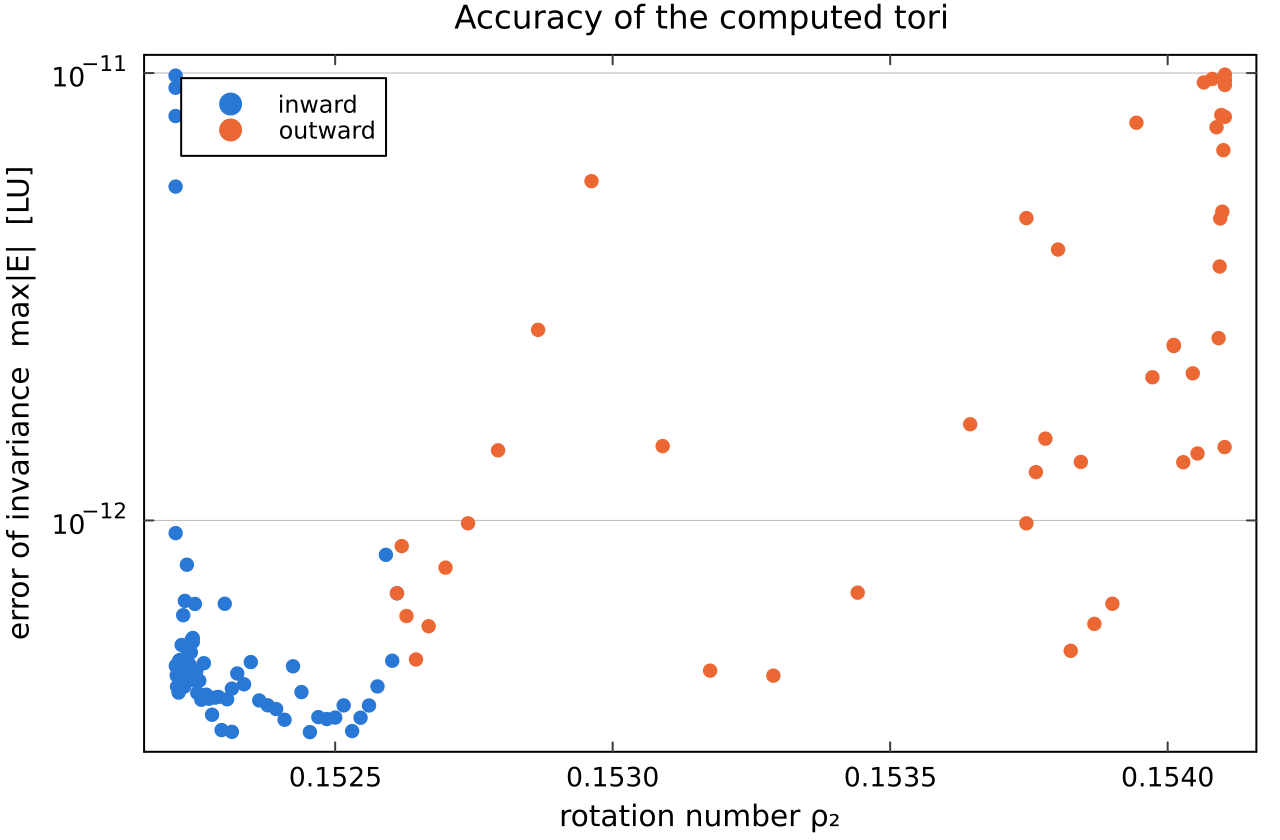
\includegraphics[width=0.6\textwidth]{id53_error.png}
\caption{Sup-norm error of invariance \eqref{eq:err} of each accepted torus of the Id~53 family,
in LU ($10^{-12}$~LU $\approx 0.24$~mm).}
\label{fig:error}
\end{figure}

\subsection{Quasi-periodic orbits in configuration space}\label{sec:qpo}
To see the tori as trajectories, we integrate the full three-degree-of-freedom flow (Julia,
Vern9, tolerance $10^{-13}$) from a point of a torus and convert the trajectory to
Enceladus-centered coordinates of the rotating frame. \Cref{fig:qpo3d} shows the QPO of the
largest Id~53 torus (radius $14.7$~km) over 30 revolutions: it stays in a thin tube around the
NRHO. \Cref{fig:qpodist} shows the distance to the NRHO over 30 periods for the tori of radius
$1.35$, $5.7$ and $14.7$~km, and \cref{fig:apolune} the crossings of the plane $y=0$ near apolune
over 300 revolutions, relative to the NRHO's crossing: cross-sections of the QPO tubes, which
fill out as the torus grows. Over the 30 revolutions the QPO of the largest torus comes no closer
than $261.0$~km to the center of Enceladus, i.e.\ it stays at least $8.9$~km above the mean
surface.

\begin{figure}[t]
\centering
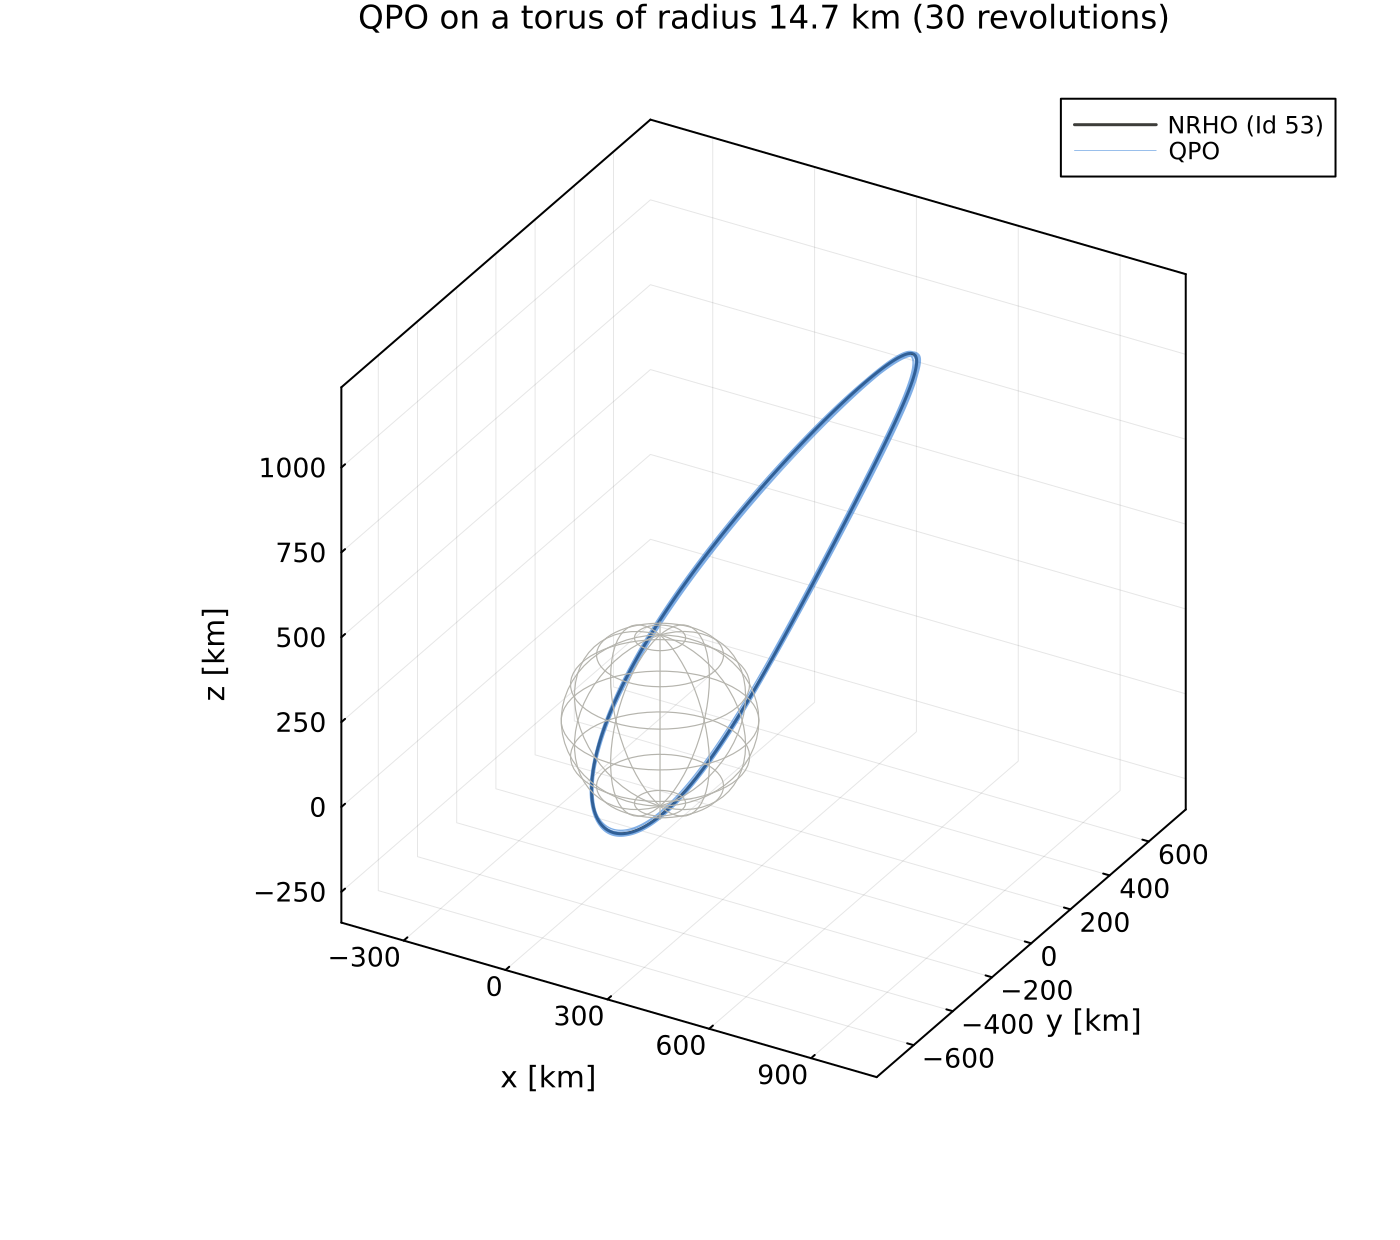
\includegraphics[width=0.65\textwidth]{id53_3d.png}
\caption{The QPO of the largest torus of the Id~53 family (radius $14.7$~km on the section) over
30 revolutions, the NRHO, and Enceladus (wireframe, radius $252.1$~km), in Enceladus-centered
rotating coordinates with equal axis scales.}
\label{fig:qpo3d}
\end{figure}

\begin{figure}[t]
\centering
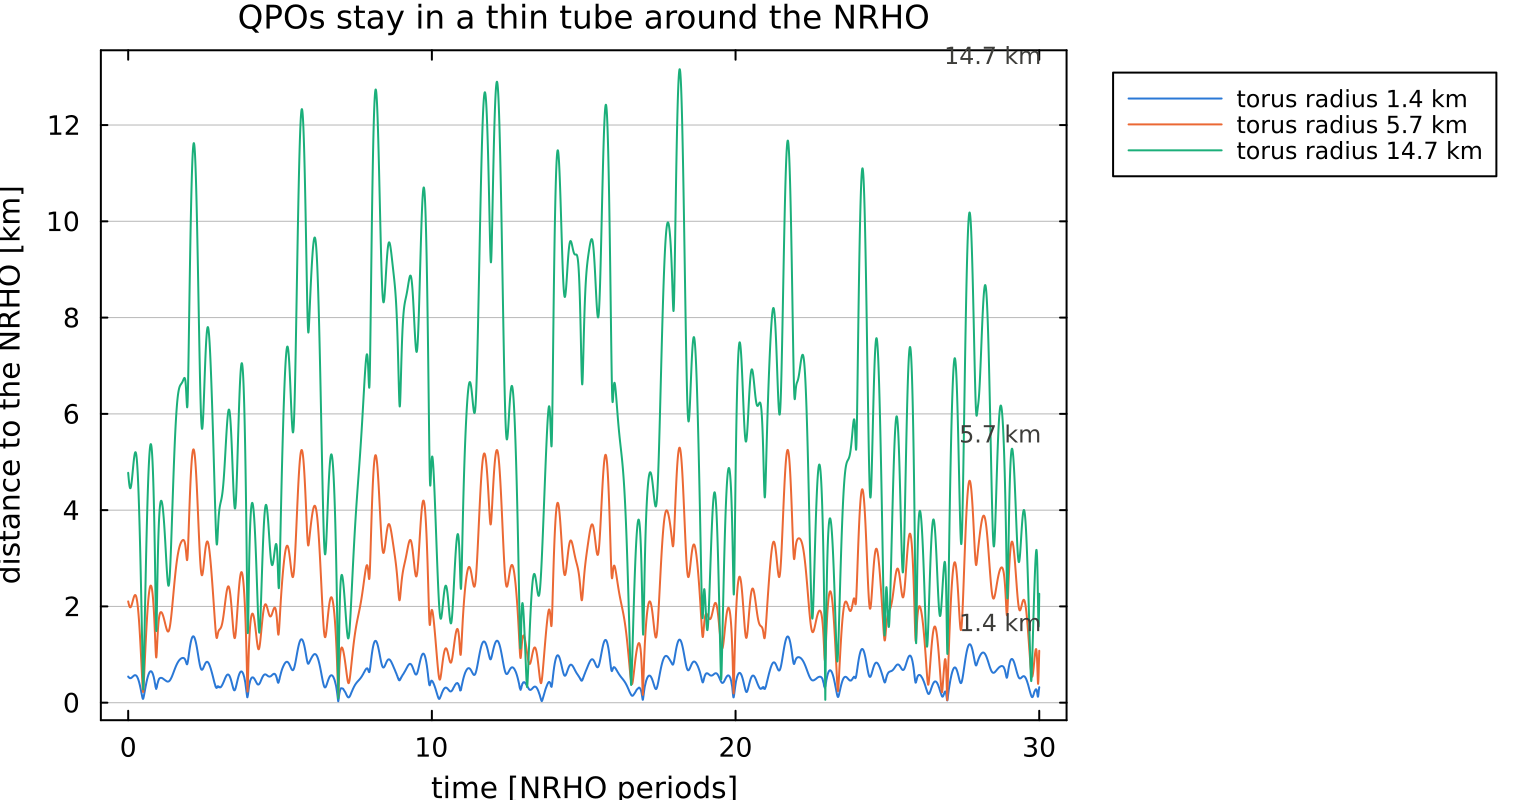
\includegraphics[width=0.85\textwidth]{id53_distance.png}
\caption{Distance from QPOs of three Id~53 tori (radius $1.35$, $5.7$ and $14.7$~km on the
section) to the NRHO (nearest point of the densely sampled periodic orbit) over 30 NRHO periods.}
\label{fig:qpodist}
\end{figure}

\begin{figure}[t]
\centering
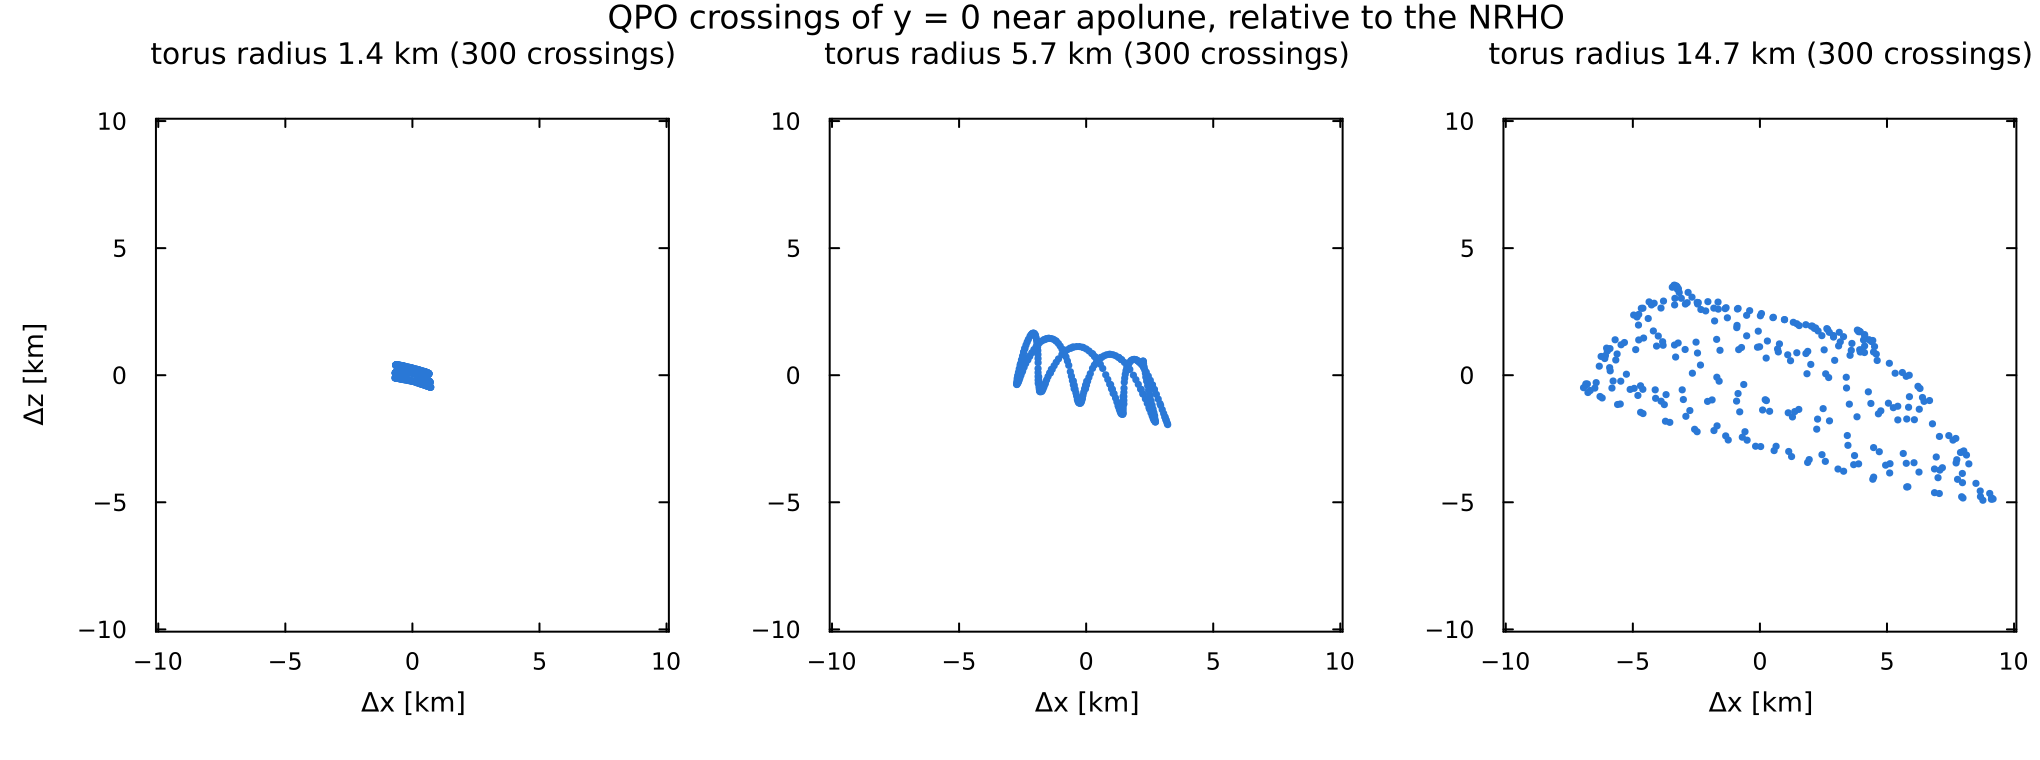
\includegraphics[width=\textwidth]{id53_apolune.png}
\caption{Crossings of the plane $y=0$ near apolune over 300 revolutions, relative to the crossing of
NRHO Id~53, for the same three tori as in \cref{fig:qpodist}.}
\label{fig:apolune}
\end{figure}

\subsection{Contrast: the family around NRHO Id~97}\label{sec:id97}
For NRHO Id~97 we continue along $\omega(\varepsilon) = \omega_s + \varepsilon\Delta\omega$ with
$\Delta\omega = \omega_s - \rho^{\mathrm{lin}} = (-2.3333\times10^{-4},-4.6605\times10^{-4})$, the
amplitude-frequency detuning of the start torus. Then $\varepsilon=-1$ is the NRHO itself
(``inward''), and $\varepsilon>0$ gives larger tori (``outward''). The family was computed in four
consecutive runs:
\begin{itemize}
\item inward, $32\times32$: 43 tori from $\varepsilon=0$ to $-0.896$, torus scale $4.9\times10^{-5}$
  to $1.6\times10^{-5}$~LU, 9 step halvings, under 10 minutes;
\item inward toward the NRHO, $32\times32$: 71 further tori, down to cumulative
  $\varepsilon=-0.980$, i.e.\ $2\%$ of the original detuning (radius $0.67$~km). The run stopped
  when the step fell below its minimum, with errors approaching $10^{-11}$; it predates the
  automatic grid refinement;
\item outward, $32\times32$: 16 tori up to $\varepsilon = 0.570$, where Newton stalls at the
  $32\times32$ truncation error (about $10^{-11}$);
\item outward with refinement: restarted from the stalled torus, Newton stalls at
  $9.9\times10^{-12}$, refines to $64\times64$ and converges to $4.3\times10^{-13}$; then 14 tori
  up to cumulative $\varepsilon=2.60$ (radius $9.4$~km) with errors $3.9\times10^{-13}$ to
  $6.6\times10^{-13}$~LU. The run ended at its prescribed limit on $\varepsilon$, not by failure.
\end{itemize}
The runs produced 144 converged tori, of which 141 are distinct (three tori appear in two
consecutive runs: the start torus and the two tori at which runs were joined). They cover
$\rho_2\in[0.19263, 0.19429]$ and radii of $0.67$ to $9.4$~km in $(q_1,q_2)$
(\cref{fig:size97}). The sup error of invariance has median $3.8\times10^{-13}$~LU on the
inward branch and $6.0\times10^{-13}$~LU on the outward branch, and maximum $1.0\times10^{-11}$~LU;
$4\times10^{-13}$~LU is about $0.1$~mm. Near the NRHO the radius grows like
$\sqrt{\rho^{\mathrm{lin}}_2-\rho_2}$, as expected for a detuning that is linear in the action.
The largest errors occur where a branch approached the limit of its grid, before refinement.

Numerically this family is as good as the Id~53 one, but physically it is limited by the low
perilune. Over 30 revolutions the QPOs of the tori of radius $0.67$, $4.8$ and $9.4$~km stay
within $0.67$, $4.6$ and $8.8$~km of the NRHO, and their minimum altitudes above the mean surface
are $+3.4$~km (torus radius $1.5$~km), $+1.7$~km ($4.8$), $+1.1$~km ($6.1$), $+0.8$~km ($6.9$) and
$-0.2$~km ($9.4$). Tori larger than about $9$~km therefore impact Enceladus, and for this member
the physically meaningful part of the family ends there regardless of the numerics.

\begin{figure}[t]
\centering
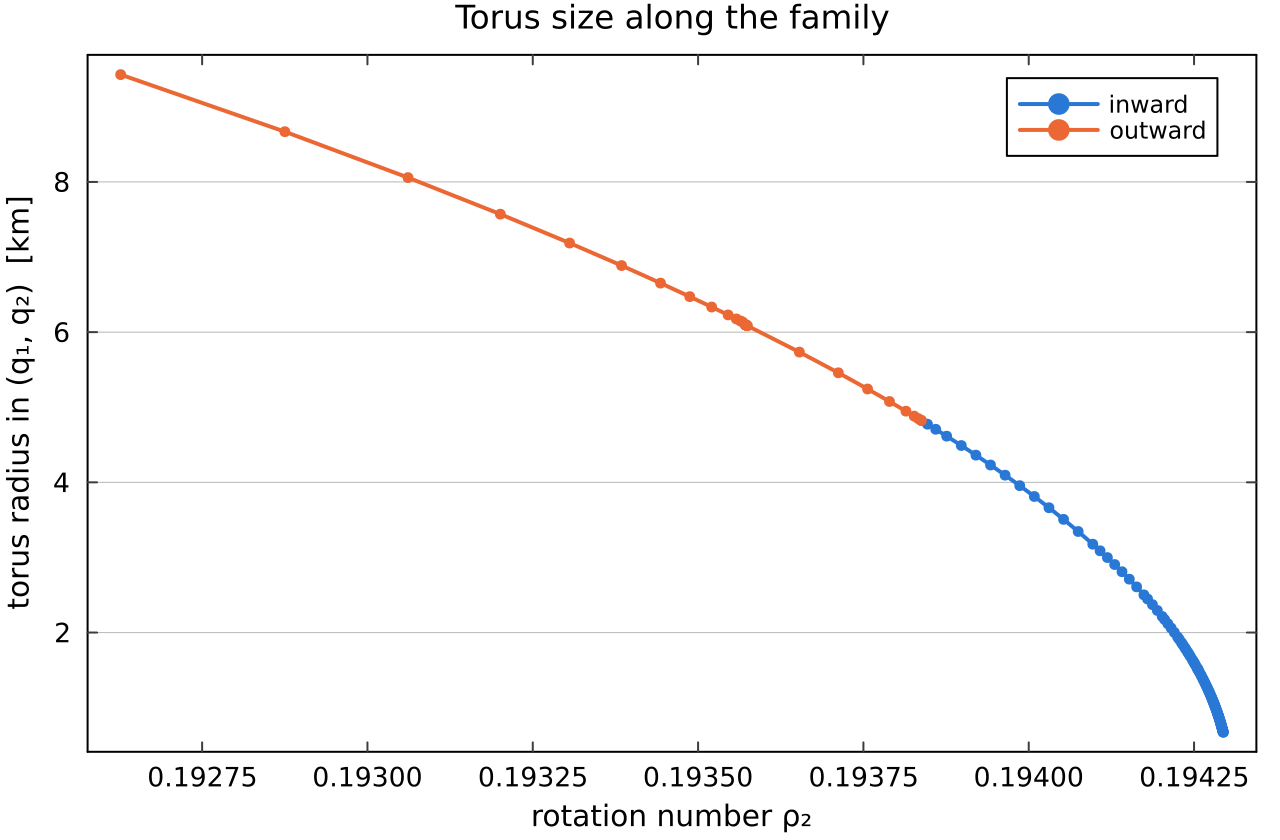
\includegraphics[width=0.55\textwidth]{id97_size.png}
\caption{Torus radius in $(q_1,q_2)$ along the Id~97 family. Tori larger than about $9$~km have
QPOs that dip below the mean surface of Enceladus.}
\label{fig:size97}
\end{figure}

\subsection{Summary over NRHO members}\label{sec:summary}
\Cref{tab:families} collects the families. The upper block lists the five main families, started
with the mode mix $(1,1)$ and continued in both directions with $\epsilon_{\mathrm{floor}} =
10^{-11}$~LU. Ids 23, 37 and 85 were set up with the same pipeline (start tori of amplitude
$4\times10^{-5}$~LU); their inward branches stopped earlier (Id~23 at a radius of $2.72$~km, Id~37
at $4.11$~km) when the continuation step fell below its minimum. Outward, every main branch first
ended near $10^{-11}$~LU on $128\times128$ grids, between $9.6$ and $14.7$~km. Restarts of the
outward branches of Ids 23, 37, 53 and 85 with anisotropic refinement and a relaxed floor of
$10^{-10}$~LU gained little: Id~23 $9.61\to9.66$~km, Id~37 $12.28\to12.4$~km, Id~53
$14.74\to15.37$~km, Id~85 $12.27\to12.35$~km, with accepted errors of at most $2.3\times10^{-11}$,
$9.8\times10^{-11}$, $7.6\times10^{-11}$ and $9.6\times10^{-11}$~LU, respectively.
\Cref{sec:limits} explains why.

The lower block lists large-torus runs. They are outward only, accepted with
$\epsilon_{\mathrm{floor}} = 10^{-10}$~LU (about $2.4$~cm, ten times the floor of the main families),
and around members chosen, with their start mode mix, where the regular region extends farthest
(\cref{sec:limits-extent}). Around NRHO Id~51 (perilune $17.6$~km), with the mix $(0.3,1)$, 27 tori
reach a radius of $20.0$~km, the largest torus we have computed; its QPOs stay at least $7.6$~km
above the surface. Around Id~87 (mix $(0.3,1)$) the $13.25$~km torus clears the surface by only
$0.8$~km, and around Id~101 (perilune $3.1$~km, mix $(1,1)$) the QPOs of the largest tori intersect
Enceladus. A second slice of the Id~37 family, with the mix $(0.3,1)$, stopped early at $7.31$~km
(steps rejected on a $32\times32$ grid at the tolerance).

The model treats Enceladus as a point mass and does not see its surface, so tori whose QPOs pass
below the mean radius are still invariant tori of the model. We keep them in the table and mark
them by a negative minimum altitude (Ids~97 and 101). Across the members the useful size of the
tori is set by the perilune altitude: Id~85 ($7.8$~km perilune) keeps a $12.3$~km torus $3.6$~km
above the surface, Id~23 a $9.6$~km torus $21.0$~km above it, while around Id~97 a $9.4$~km torus and
around Id~101 a $14.0$~km torus reach $0.2$ and $3.4$~km below it.

\begin{table}[t]
\centering
\caption{Families of Lagrangian tori around eight NRHO members. Errors are sup-norm invariance
errors \eqref{eq:err} in LU (median inward / outward, or outward only; maximum). Tori: distinct
converged tori. Radius: on the section, in $(q_1,q_2)$. Minimum QPO altitude: over 30 revolutions
from the largest torus, above the $252.1$~km mean radius. \emph{QPOs that intersect the surface are
included}, marked by a negative minimum altitude and $\dagger$; the point-mass model does not see
the surface. Upper block: start mode mix $(1,1)$, $\epsilon_{\mathrm{floor}}=10^{-11}$~LU; radii
include the outward extensions with $\epsilon_{\mathrm{floor}}=10^{-10}$~LU (Id~53: $+35$ tori),
whose errors are not in the error column (see text); $^{a}$minimum altitude of the largest torus
before the extension (radius $9.61$, $12.28$, $14.7$ and $12.27$~km). Lower block: large-torus runs,
outward only, $\epsilon_{\mathrm{floor}}=10^{-10}$~LU ($\approx2.4$~cm), start mode mix as listed.}
\label{tab:families}
\small
\setlength{\tabcolsep}{3.5pt}
\begin{tabular}{rcccccc}
\toprule
Id (mix) & perilune & $\rho^{\mathrm{lin}}$ & tori & radius & median / max error & min.\ QPO \\
   & alt.\ (km) &                     &      & (km)   & (LU)               & alt.\ (km) \\
\midrule
23 & 25.8 & $(0.336377, 0.101653)$ & 74 & 2.72--9.66 & $6.9\mathrm{e}{-13}$ / $4.5\mathrm{e}{-12}$; $1.0\mathrm{e}{-11}$ & $+21.0^{a}$ \\
37 & 21.8 & $(0.337056, 0.128252)$ & 55 & 4.11--12.4 & $7.4\mathrm{e}{-13}$ / $1.2\mathrm{e}{-12}$; $1.0\mathrm{e}{-11}$ & $+15.6^{a}$ \\
53 & 17.1 & $(0.339096, 0.152183)$ & 109 & 1.35--15.37 & $4.5\mathrm{e}{-13}$ / $1.9\mathrm{e}{-12}$; $9.9\mathrm{e}{-12}$ & $+8.9^{a}$ \\
85 &  7.8 & $(0.348321, 0.185508)$ & 75 & 1.04--12.35 & $3.6\mathrm{e}{-13}$ / $2.1\mathrm{e}{-12}$; $1.0\mathrm{e}{-11}$ & $+3.6^{a}$ \\
97 &  4.2 & $(0.353958, 0.194304)$ & 141 & 0.67--9.4 & $3.8\mathrm{e}{-13}$ / $6.1\mathrm{e}{-13}$; $1.0\mathrm{e}{-11}$ & $-0.2^{\dagger}$ \\
\midrule
51 $(0.3,1)$ & 17.6 & $(0.338768, 0.149597)$ & 27 & 3.59--20.01 & $6.4\mathrm{e}{-13}$; $9.9\mathrm{e}{-11}$ & $+7.6$ \\
87 $(0.3,1)$ &  7.2 & $(0.349137, 0.187041)$ & 27 & 3.48--13.25 & $1.8\mathrm{e}{-12}$; $1.0\mathrm{e}{-10}$ & $+0.8$ \\
101 $(1,1)$  &  3.1 & $(0.356035, 0.196740)$ & 27 & 5.30--14.01 & $2.7\mathrm{e}{-12}$; $9.5\mathrm{e}{-11}$ & $-3.4^{\dagger}$ \\
37 $(0.3,1)$ & 21.8 & $(0.337056, 0.128252)$ & 22 & up to 7.31 & --- & --- \\
\bottomrule
\end{tabular}
\end{table}

\subsection{Cost}
Each Newton step evaluates the section map and its differential at every grid point, i.e.\ $N$
integrations of the variational equations over about one NRHO period; this dominates the cost of
a step, while the cohomological equations and frame construction are FFT-based and comparatively
cheap. The evaluations are independent, and we run them in parallel with OpenMP. One Newton solve
of the Id~97 start torus on $32\times32$ (two error evaluations and one step) takes $5.0$~s on one
thread and $0.53$~s on 12 threads ($9.4\times$), with identical errors; compiling with
optimization (\texttt{-O2}) reduces the single-thread time from $5.20$ to $1.76$~s ($3.0\times$),
and the two gains multiply. A Newton step on a $32\times32$ grid therefore takes well under a
second. On $128\times128$ grids, with $16384$ map evaluations per step, this is the difference
between minutes and seconds. The first inward Id~97 run (43 tori, 171 evaluations of the
invariance error including rejected steps), made with the serial, unoptimized build, took under 10
minutes. \todo{Machine and CPU model; timing per step on $128\times128$.}
For comparison, the dense collocation Newton step costs $O((4N)^3)$ operations and storage
$O((4N)^2)$.


%% ============================================================================
\section{Limits of the torus families and their breakdown}\label{sec:limits}
Every outward branch of \cref{tab:families} ended on a small continuation step, and restarting it
with finer or anisotropic grids and a looser tolerance floor moved its end by at most
$0.6$~km. This section shows that the families end close to the edge of the regular region
around their NRHO, where the tori approach breakdown, and that for low-perilune members the
surface of Enceladus comes first. We measure the regular region directly with orbits of $F$
(\cref{sec:limits-extent}), describe two signatures of the approach to breakdown
(\cref{sec:limits-drift,sec:limits-modes}), and explain how the solver responds to them
(\cref{sec:limits-response}), why the direction of continuation matters
(\cref{sec:limits-direction}), and where the physical edge lies (\cref{sec:limits-surface}).

\subsection{How large can the tori get?}\label{sec:limits-extent}
For each of the 29 elliptic members with perilune above the surface we grow orbits of $F$ from the
fixed point along three mode mixes, $z^* + a\,(c_1\mathrm{Re}\,V_1 + c_2\mathrm{Re}\,V_2)$ with
$(c_1,c_2) = (1,1)$, $(1,0.3)$ and $(0.3,1)$ and increasing amplitude $a$ (successive amplitudes
differ by a factor of about $1.15$). An orbit is called regular if the NAFF rotation numbers of
the two halves of $4096$ iterates agree to $10^{-7}$ (\cref{sec:guess}). For each mix we record the
largest regular amplitude and the maximum distance of that orbit from the NRHO on the section, the
\emph{extent} of the regular region in that direction (\cref{fig:extent}). The extent reaches at
most about $16$ to $21$~km: Id~101 $21.4$~km along $(1,1)$, Id~87 $17.9$~km, Id~97 $17.6$~km,
Id~37 $16.7$~km and Id~51 $16.3$~km along $(0.3,1)$, and Id~53 $15.9$~km along $(1,1)$. It varies
strongly between members and between mixes. Around Id~51 it is $16.3$~km along $(0.3,1)$ but
$8.9$~km along $(1,1)$ and $4.4$~km along $(1,0.3)$; around Ids~59 and 71, which lie close to
low-order resonances (\cref{tab:scan}), no orbit of the sweep is regular in some directions. It
does not follow the perilune altitude.

The extent is an estimate. It is resolved only to the amplitude step and in three directions, and
it measures the distance of an orbit from the NRHO rather than the radius of a torus about its own
centre. The largest torus around Id~51 ($20.0$~km) is in fact larger than the extent found along
$(0.3,1)$, and the finer sweep of \cref{fig:drift} finds regular orbits up to $19.2$~km in that
direction. Still, the largest computed tori of the main families lie close to the extent around
their NRHO (Id~53: $15.37$ against $15.9$~km; Id~85: $12.35$ against $13.2$~km), and tori larger than
about $20$~km are not to be expected around these NRHOs.

\begin{figure}[t]
\centering
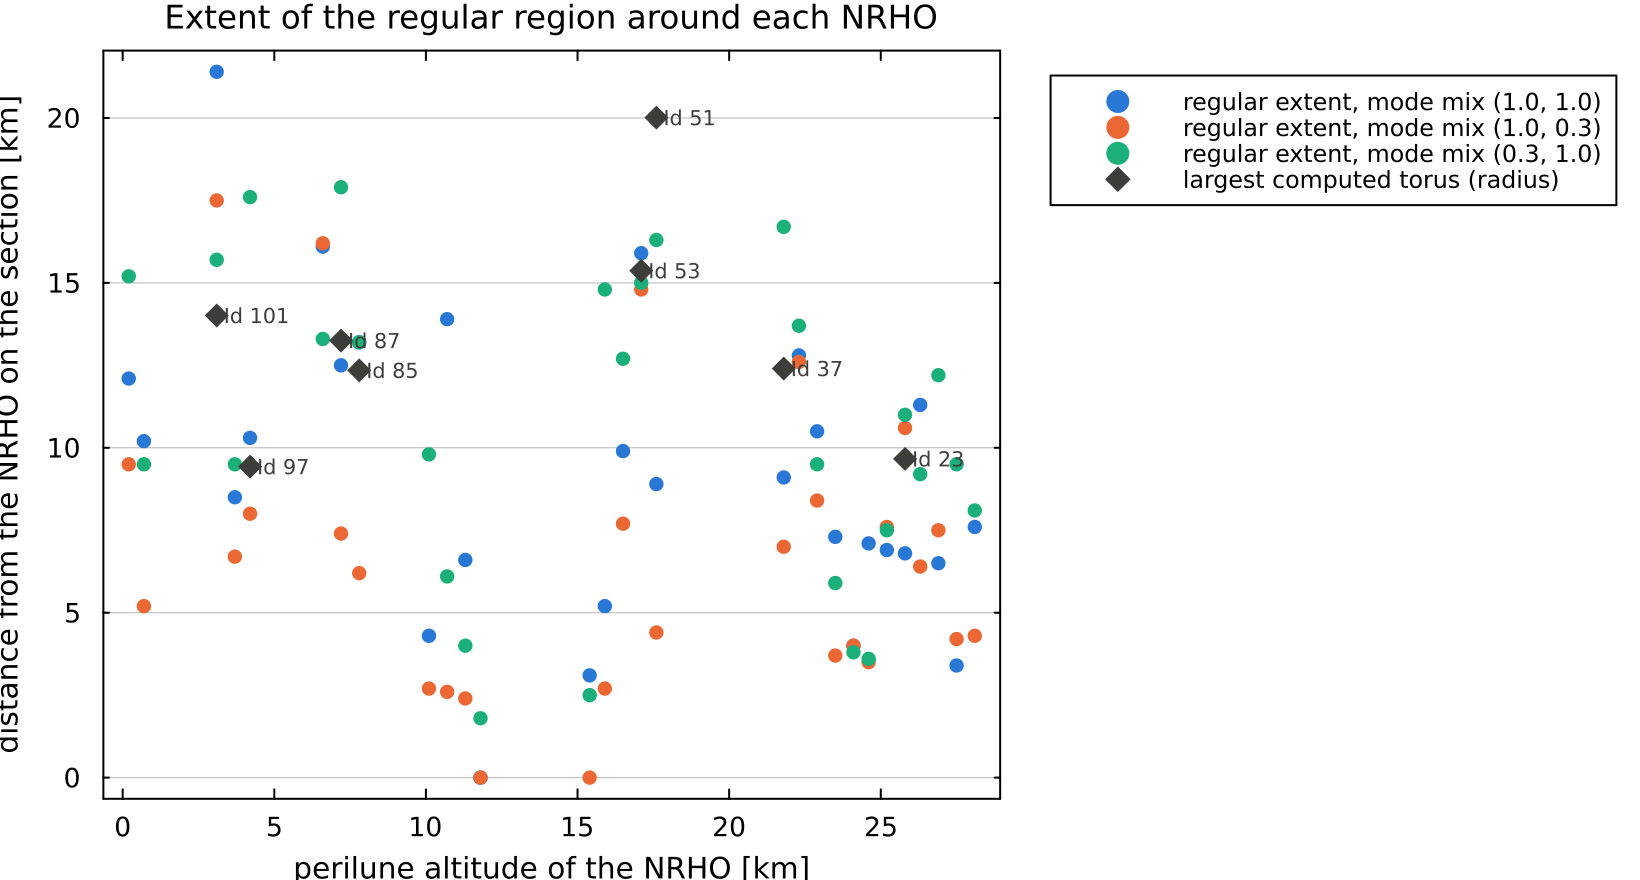
\includegraphics[width=\textwidth]{limits_extent.png}
\caption{Extent of the regular region around each elliptic NRHO with perilune above the surface:
the maximum distance from the NRHO, on the section, of the largest regular orbit of the sweep along
each of three mode mixes, against the perilune altitude. Diamonds: radius of the largest computed
torus of each member. Source: \nolinkurl{results/families/stability_edge_scan.txt}.}
\label{fig:extent}
\end{figure}

\subsection{First signature: loss of regularity}\label{sec:limits-drift}
\Cref{fig:drift} shows the frequency drift between the two orbit halves along finer sweeps for
Id~53 (mix $(1,1)$) and Id~51 (mix $(0.3,1)$). Up to about $12$~km from the NRHO the drift stays
between $10^{-11}$ and a few $10^{-9}$. It then rises, with isolated excursions (Id~51:
$1.1\times10^{-7}$ at $12.8$~km, back to $3\times10^{-10}$ at $16.6$~km), and crosses the regularity
threshold $10^{-7}$ for good near $20$~km: Id~53 has a drift of $3.3\times10^{-7}$ at $21.2$~km and
$2.4\times10^{-4}$ at $31.0$~km, Id~51 $2.4\times10^{-3}$ at $22.5$~km. Beyond about $22$~km (Id~51)
and $31$~km (Id~53) the orbits escape Enceladus: the next amplitudes of the sweeps reach distances
of about $4.8$ to $5.0\times10^{5}$~km (e.g.\ $486{,}700$~km for Id~53).

\begin{figure}[t]
\centering
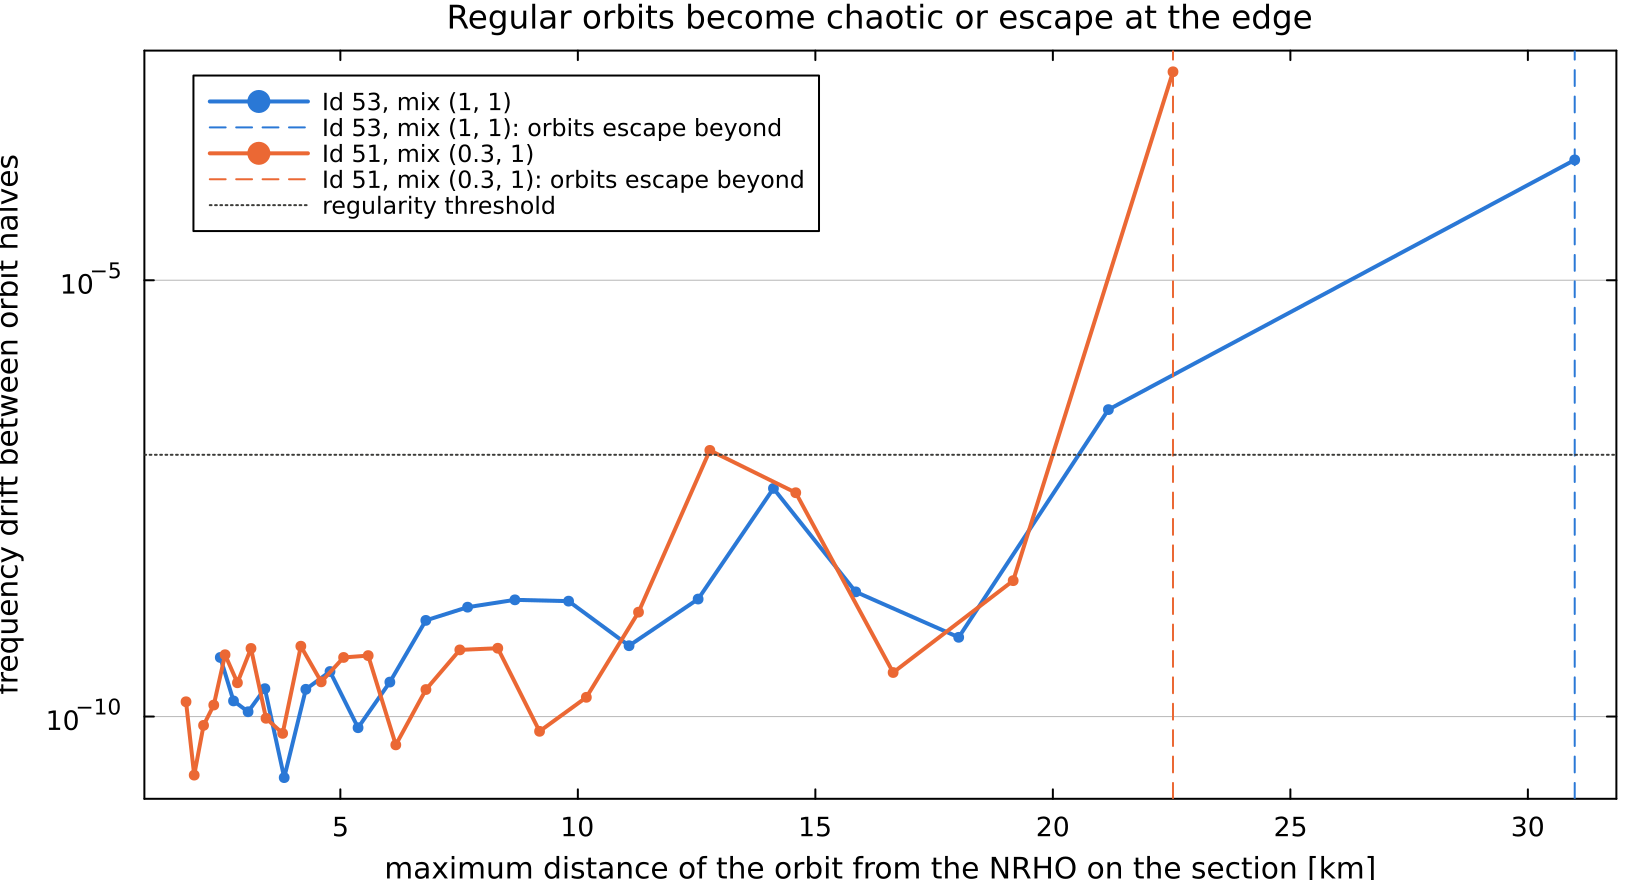
\includegraphics[width=\textwidth]{limits_drift.png}
\caption{Frequency drift between the two halves of orbits of $4096$ iterates, against the maximum
distance of the orbit from the NRHO on the section, for sweeps around NRHO Id~53 (mix $(1,1)$) and
Id~51 (mix $(0.3,1)$). Dotted: the regularity threshold $10^{-7}$. Dashed: beyond these distances
the orbits escape Enceladus.}
\label{fig:drift}
\end{figure}

\subsection{Second signature: growth of the Fourier content}\label{sec:limits-modes}
\Cref{fig:modes} shows, for every torus of the Id~53 and Id~51 families, the highest Fourier mode
$|k_j|$ in each angle with a coefficient above $10^{-11}$~LU, the accuracy of the solve. Up to a
radius of about $12$~km the tori need only a few modes, mostly $4$ to $10$ (at most $14$). Then the
number grows rapidly and anisotropically: around Id~53 to about $60$ by $15$~km, and around Id~51
to $127$ in $\theta_2$ and $63$ in $\theta_1$ at $20.0$~km, on a $256\times512$ grid, i.e.\ up to the
filter cutoff $n_j/4$ in both angles. Along the Id~51 family the grid grows accordingly, from
$32\times32$ through $32\times128$, $64\times256$ and $128\times256$ to $256\times512$. A torus
approaching breakdown loses smoothness: its Fourier coefficients decay ever more slowly, and the
number of modes needed for a given accuracy grows without bound. The growth in
\cref{fig:modes} is this approach to breakdown of the KAM tori, seen in the same members and at the
same distances as the loss of regularity of \cref{fig:drift}; it is not only a numerical limit of
the solver. The spike at radii near $1.4$~km is not part of this picture: the innermost Id~53 tori
were accepted close to the tolerance floor, and their coefficients carry noise at the $10^{-11}$
level, which the count picks up.

\begin{figure}[t]
\centering
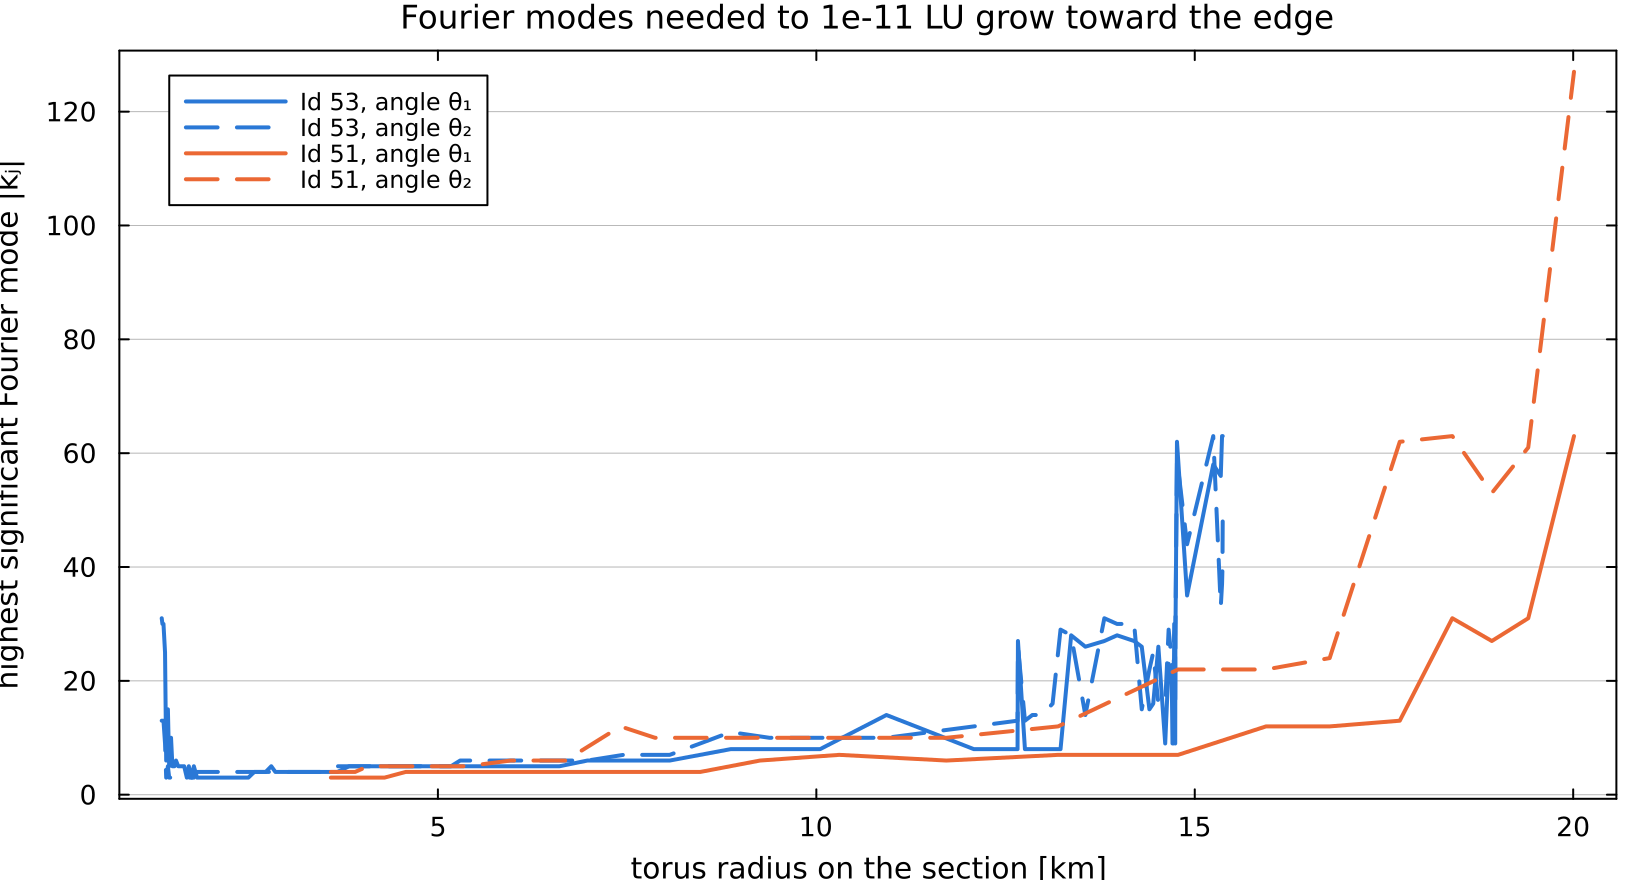
\includegraphics[width=\textwidth]{limits_modes.png}
\caption{Highest Fourier mode $|k_j|$ with a coefficient above $10^{-11}$~LU, per angle, against
the torus radius, for the Id~53 (mix $(1,1)$) and Id~51 (mix $(0.3,1)$) families. The spike near
$1.4$~km comes from the innermost Id~53 tori, accepted near the tolerance floor, which carry noise
at that level.}
\label{fig:modes}
\end{figure}

\subsection{How the computation responds}\label{sec:limits-response}
The growth of the Fourier content is what stopped the original outward branches. All of them ended
near $10^{-11}$~LU on $128\times128$ grids. The error spectrum of the last Id~53 outward torus
(radius $14.7$~km) is concentrated at $k=(-31,6\ldots8)$, i.e.\ at $|k_1| = 31$, just below the
filter cutoff $n_1/4 = 32$ in $\theta_1$, and is at about $10^{-15}$ elsewhere. This is truncation in
$\theta_1$ alone, not noise of the map: a relative threshold on the right-hand sides of the
cohomological equations, varied from $10^{-10}$ to $10^{-4}$, had no effect at all. Refining both
angles, as in \cref{sec:practical}, quadruples the cost and soon reaches the grid cap; the
truncated angle is what needs refining. We therefore refine anisotropically: the solver measures,
per angle, the fraction of the error spectrum in the band $3n_j/16\le|k_j|<n_j/4$ and doubles only
the angle(s) in which that fraction is at least $20\%$. For the edge torus of Id~53 ($128\times128$,
$9.92\times10^{-12}$~LU) the fractions are $60\%$ ($\theta_1$) and $13\%$ ($\theta_2$). Refined to
$256\times128$ its error goes $9.93\times10^{-12}$, $4.62\times10^{-12}$, $3.20\times10^{-12}$, while
on $128\times128$ the step made it worse ($2.5\times10^{-11}$).

Two refinements of this rule turned out to be necessary once the floor was relaxed to
$10^{-10}$~LU and the grid cap raised to $262144$ points. First, refinement must require that the
\emph{best} torus is truncated: otherwise steps whose predictor had left the basin were refined
instead of halved (Id~37 was refined to $128\times2048$ with $0.003\%$ of its error near the cutoff,
Id~85 to $512\times512$ from an iterate at $1.5\times10^{-8}$). Second, a branch whose tori are
accepted just below the floor on a grid that truncates them never stalls, so refinement on stall
never triggers, while the step shrinks indefinitely; Id~87 sat on a $32\times64$ grid with accepted
errors of $1.0\times10^{-10}$ and 25 step halvings. After an accepted torus whose error exceeds
$0.3\,\epsilon_{\mathrm{floor}}$ the grid is now refined before the next step (proactive refinement).

With these changes the extensions of the main families still gained little: Id~53 went from
$14.74$ to $15.37$~km, and Ids~23, 37 and 85 by about $0.1$~km or less (\cref{sec:summary}), even
though, with the corrected rule, the last tori of Ids~23 and 85 genuinely required $512\times512$
grids (their best tori had most of their error spectrum just below the cutoff). This is
what \cref{fig:extent,fig:drift,fig:modes} predict: the families had already reached the edge of the
regular region, where each further kilometre costs a large increase in the number of modes. The
remaining progress of a branch is limited by breakdown, not by the accuracy of the map.

\subsection{Direction in the two-parameter family}\label{sec:limits-direction}
Lagrangian tori of a 4D map at fixed energy form a two-parameter family, and continuation along a
line in $\omega$ follows one path through it (\cref{sec:practical}). The path is set by the start
torus, i.e.\ by the mode mix of the orbit it is fitted to, and the regular region is far from
round (\cref{sec:limits-extent}). Starting in the mix in which the region extends farthest pays
off: around Id~51, whose extent along $(1,1)$ is only $8.9$~km, the start torus with the mix
$(0.3,1)$ leads to a family that reaches $20.0$~km, the largest torus computed, against $15.4$~km
for Id~53 along $(1,1)$. \Cref{fig:apo51} shows the QPOs of three Id~51 tori at apolune: the tube of
the $20.0$~km torus spans about $25\times10$~km there.

\begin{figure}[t]
\centering
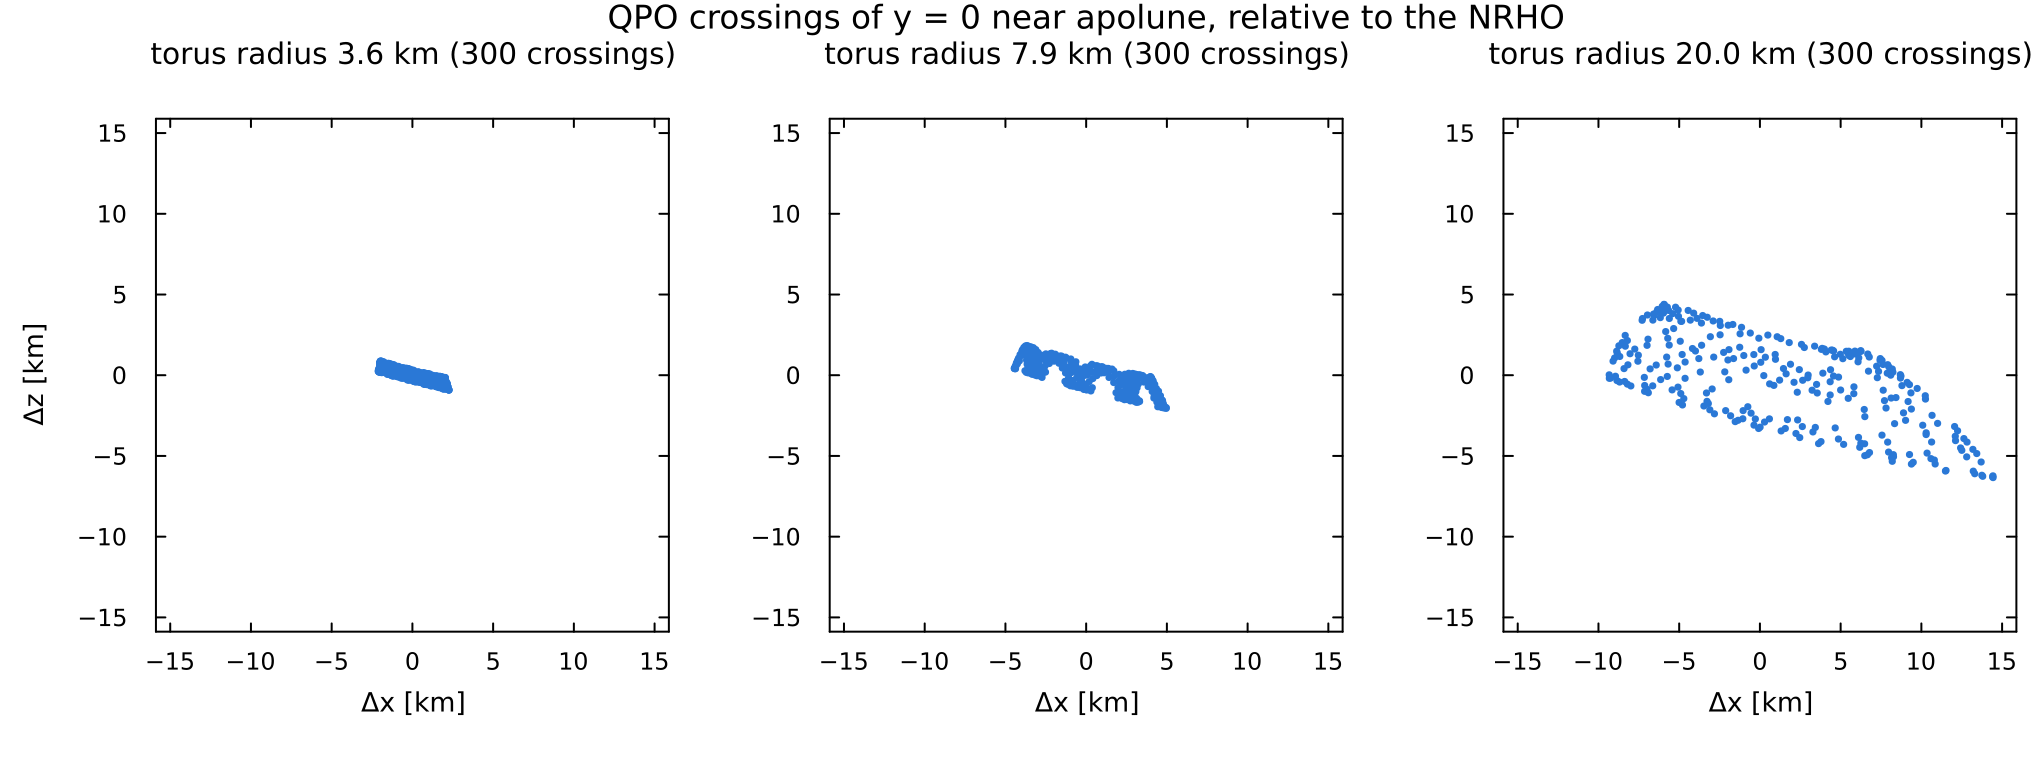
\includegraphics[width=\textwidth]{id51_apolune.png}
\caption{Crossings of the plane $y=0$ near apolune over 300 revolutions, relative to the crossing of
NRHO Id~51, for three tori of the Id~51 family with mix $(0.3,1)$ (radius $3.6$, $7.9$ and
$20.0$~km on the section).}
\label{fig:apo51}
\end{figure}

\subsection{Physical edge: intersection with the surface}\label{sec:limits-surface}
The CR3BP treats Enceladus as a point mass, so the model does not see its surface: a torus whose
QPOs pass below the mean radius is still an invariant torus of the model, but not a usable orbit.
We keep such tori and mark them (\cref{tab:families}). Over 30 revolutions from the largest torus
of each run, the minimum altitude above the $252.1$~km mean radius is $-0.2$~km for Id~97 (torus
radius $9.4$~km), $-3.4$~km for Id~101 ($14.0$~km), $+0.8$~km for Id~87 ($13.25$~km) and
$+7.6$~km for Id~51 ($20.0$~km). For the low-perilune members the surface therefore ends the useful
part of the family well inside the regular region: Id~101 has the largest extent of all members,
$21.4$~km, but its QPOs reach $3.4$~km below the surface already at $14.0$~km. For the higher
members, such as Ids~51 and 53, the regular region ends first.

%% ============================================================================
\section{Discussion}\label{sec:discussion}

\subsection{Convergence where the hypotheses hold}
Once the numerical issues of \cref{sec:lessons} were addressed, the method behaved as the theory
says. On the twist map the error squares at each step. On the CR3BP, an orbit-fitted torus with
error $10^{-10}$~LU is corrected to the map-noise floor in one step, and along the family the
secant predictor plus two or three quasi-Newton steps suffice, each step costing $N$ map
evaluations and $O(N\log N)$ operations. The torsion is symmetric and non-degenerate, the frame
check is small, and the linearized residual is a small fraction of the error, all of which are
a-posteriori indicators of the hypotheses of the KAM theorem
\cite{figueras2017rigorous}. These indicators were also how the problems were found: a
linearized residual comparable to the error, a non-symmetric $\avg{T}$, or a large frame check
each pointed at a specific defect in the implementation. We have not attempted a computer-assisted
proof; the a-posteriori theorems \cite{figueras2017rigorous,haro2016book} would require rigorous
enclosures of the Poincar\'e map, for instance with $C^r$-Lohner methods
\cite{wilczak2007lohner}.

\subsection{Lessons: numerical hygiene for small tori far from the origin}\label{sec:lessons}
The Barcelona KAM code was designed for maps on $\T^d\times\R^d$ such as the standard and
Froeschl\'e maps, where tori are homotopic to the zero section and of order one. In that setting
its choices are natural. Several of them become problems for Cartesian tori of radius
$10^{-5}$~LU at $|z|\approx 1$; we list them because they are likely to affect other applications
in astrodynamics.
\begin{itemize}
\item \emph{Angle lift.} For tori on $\T^d\times\R^d$ only $K(\theta)-(\theta,0)$ is periodic. For
  Cartesian tori no lift applies; leaving it in produced an $O(1)$ spurious error.
\item \emph{Frame choice.} A constant transversal field cannot be used around an elliptic point
  (\cref{sec:verification}); the metric frame \eqref{eq:frame} can. In the original coordinates the
  metric induced from $\R^6$ on the section is ill-conditioned ($|\nabla p_3|\sim 50$--$100$), and
  the tori are so eccentric that $L^\top L$ is nearly singular in places; the resulting $B$ and $N$
  are poorly resolved on the grid. Torus-adapted symplectic coordinates with $G=I$ remove both
  problems. An earlier, isotropic rescaling made the twist look weak, which was an artifact of the
  coordinates: the torsion is intrinsic once the action is measured by $\Omega$.
\item \emph{Absolute thresholds.} With tori of radius $10^{-5}$, the right-hand side of the
  normal-row cohomological equation was of order $10^{-15}$, and an absolute small-coefficient
  threshold of $10^{-17}$ dropped about $85\%$ of it, so each step left a residual of the size of
  the error. Rescaling to unit circles and making the threshold relative fixed this.
\item \emph{Nyquist modes.} One-sided Nyquist coefficients made $DK$, $N$ and $T$ complex in real
  space, and routines that use only the real part silently dropped the imaginary parts.
\item \emph{Error norm.} The Fourier $\ell^1$ norm of $E$ sums a broadband floor of about
  $10^{-14}$ per coefficient. It reported about $10^{-11}$ on $32\times32$ and $1.6\times10^{-10}$
  on $128\times128$ for a torus whose sup error was $5.4\times10^{-13}$~LU. This made refined grids
  look worse and stalled continuation; with the sup norm, refinement behaves as expected.
\item \emph{Stale frame.} With local coordinates built once from the start torus, continuation
  stalled after $|\Delta\varepsilon|\approx0.1$; rebuilding them from each accepted torus removed
  the stall (a restart from the stuck torus converged at once, to $5.5\times10^{-13}$).
\end{itemize}
In addition, the state transition matrix was read transposed and the gradient of $p_3$ missed the
chain-rule factor in the problem-specific interface code; the Jacobian check and the fixed-point
Newton test catch both kinds of error. None of these issues is a flaw of the method. They are the
practical cost of moving a validated code to a problem with very different scales, and the
diagnostics above are a cheap way to detect them.

\subsection{Limitations}\label{sec:limitations}
\begin{itemize}
\item \emph{Map-noise floor.} Converged tori have sup errors of about $4\times10^{-13}$~LU. The
  spectrum of $E$ shows a broadband floor of about $10^{-14}$ per coefficient, plus peaks at the
  filter cutoff and at the near-resonant mode $k=(-1,7)$. Tightening the section tolerance from
  $10^{-12}$ to $10^{-14}$ was necessary; an earlier, larger floor did not move with the RK78
  tolerance or the section tolerance beyond that. The exact source of the remaining floor in the
  map evaluation is not yet characterized. \todo{Characterize the floor (e.g., by comparing with an
  extended-precision or Taylor integrator).}
\item \emph{Outer edge of the families.} The outer end of the Id~53 family is not a limit of
  the map accuracy, as we first thought, but close to the edge of the regular region around the
  NRHO (\cref{sec:limits}). The error at the end of the original branch was truncation in one
  angle; anisotropic refinement removes it, but the number of Fourier modes the tori need grows
  rapidly toward the edge, so each further kilometre is expensive and the extensions gained only
  $0.6$~km. Beyond the edge, orbits become chaotic or escape. Tori larger than about $20$~km are
  not expected around the members we scanned; reaching the last regular tori would need very
  large grids or a method adapted to the approach to breakdown. The more accurate map evaluation or
  the flow-map/multiple-shooting formulation of Haro and Mondelo \cite{haromondelo2021flow} can
  lower the error floor, but not move the edge of the regular region.
\item \emph{Physical edge: surface intersection.} For low-perilune members the family ends
  physically before it ends dynamically. Around NRHOs Id~97 (perilune $4.2$~km) and Id~101 ($3.1$~km)
  the QPOs of the larger tori pass below the mean surface of Enceladus, and members with
  Id~$\ge113$ have perilunes below it. Since the point-mass model does not see the surface, we keep
  these tori and mark them (\cref{tab:families,sec:limits-surface}). The scan of \cref{sec:scan} is
  therefore part of the method for this problem: perilune altitude, as well as resonance distance
  and the extent of the regular region, decides which members are worth continuing. Altitudes here
  are measured from the $252.1$~km mean radius.
\item \emph{Resonances.} The line in $\omega$ crosses resonances densely; numerically only
  low-order ones with small divisors on the grid matter. Near the $1{:}2$ resonance (NRHO Id~72)
  the method is not applicable to the resonant tori, which are not Lagrangian KAM tori with the
  prescribed frequencies. The quasi-Newton step also amplifies noise through the small divisors,
  which is why stall detection is needed. We have not checked Diophantine conditions.
\item \emph{Poincar\'e map vs.\ flow map.} We use a Poincar\'e map at fixed energy, which yields a
  symplectic map of the right dimension. Haro and Mondelo note that the time-$T$ flow-map approach
  gives exact symplectic maps in both isochronous and isoenergetic settings and is cheaper to code
  and evaluate, and that Poincar\'e maps complicate multiple shooting
  \cite[Remark~2.4.5, pp.~8--9]{haromondelo2021flow}. Multiple shooting would also shorten the
  integration intervals, which may help near the close passage of the NRHO over Enceladus. A flow-map version of this framework
  \cite{haromondelo2021flow,fernandezmora2024siads,fernandezmora2026convergence} is a natural next
  step.
\item \emph{Tolerance of the large-torus runs.} The large-torus runs and the extensions of the
  main families were accepted with $\epsilon_{\mathrm{floor}} = 10^{-10}$~LU (about $2.4$~cm), ten
  times the floor of the main families; their median errors are still between $6.4\times10^{-13}$ and $2.7\times10^{-12}$~LU.
  The Id~37 slice with the mix $(0.3,1)$ stopped at $7.31$~km, well short of the $16.7$~km extent
  in that direction, and could be restarted.
\item \emph{Extent of the Id~97 family.} The inward branch stopped at $2\%$ of the original
  detuning on $32\times32$, before automatic refinement existed, and the outward branch stopped at
  its prescribed limit $\varepsilon = 2.60$ (radius $9.4$~km), which is already beyond the impact
  boundary. \todo{Report the end point of the far-outward Id~97 run (was still running), or drop
  it, since those tori impact Enceladus.}
\item \emph{Stability information.} We have not yet computed the linear stability of the tori
  (the tangent and normal bundles beyond the frame), nor mission-relevant properties beyond the
  minimum altitude (eclipse, station-keeping cost). \todo{Decide whether to include any of
  these for the conference version.}
\end{itemize}

%% ============================================================================
\section{Conclusions}\label{sec:conclusions}
We built a parameterization-method solver for Lagrangian invariant tori of the Saturn--Enceladus
CR3BP around nearly stable NRHOs, based on the KAM code of Haro and Luque and the RTBP library of
Haro and Mondelo, and verified it on an integrable twist map with exact solutions and against
finite differences and an independent dense Newton solver. With torus-adapted symplectic
coordinates, scale-free thresholds, a sup-norm error, low-pass filtering, stall detection and grid
refinement, the quasi-Newton step converges from orbit-fitted guesses to the noise floor of the
Poincar\'e map in one to three steps, at $O(N\log N)$ cost plus $N$ map evaluations per step.
Along the elliptic NRHO members the perilune altitude falls from $28$~km to below the surface, so
members must be selected by perilune altitude as well as by distance to low-order resonances.
Continuation in the rotation vector produced a family of 109 tori around NRHO Id~53 (perilune
$17.1$~km), with radii from $1.35$ to $14.7$~km on the section, median errors of
$4.5\times10^{-13}$ and $1.9\times10^{-12}$~LU and a maximum of $9.9\times10^{-12}$~LU; its QPOs
stay at least $8.9$~km above Enceladus, and an extension with a floor of $10^{-10}$~LU reaches
$15.37$~km. Around NRHO Id~97 (perilune $4.2$~km) a family of 141 tori, from $0.67$ to
$9.4$~km, is equally accurate, but its tori larger than about $9$~km impact Enceladus. Families
around Ids~23, 37 and 85, and large-torus runs around Ids~51, 87 and 101, complete the picture; with
a start torus in the mode mix $(0.3,1)$ the Id~51 family reaches $20.0$~km, the largest torus
computed, with QPOs at least $7.6$~km above the surface.

The families end close to the edge of the regular region around their NRHO, which orbit sweeps
place at most about $16$ to $21$~km from the NRHO on the section, with strong variation between
members and directions. Near that edge the frequency drift of orbits crosses the regularity
threshold and the Fourier content of the tori grows rapidly and anisotropically, the approach to
breakdown of the tori. Anisotropic and proactive grid refinement follow this growth, but gain
little: the outer edge is dynamical rather than numerical. For low-perilune members the surface of
Enceladus comes first, and we keep and mark the tori whose QPOs intersect it. Next steps are the
stability of the tori, the Id~37 slice and the Id~101 family toward their regular extents, and the
use of the tori in mission design for an Enceladus orbiter.

\paragraph{Code and data availability.} \todo{Repository URL (github.com/jared711/nrho-lagrangian-tori?),
license (the RTBP library is LGPL v3 or later), and the commit used for the results; the tori,
run logs and commands are in \nolinkurl{results/families/nrho_id<Id>/} (large-torus runs in
\nolinkurl{mix_*} subdirectories), the member scan in
\nolinkurl{results/families/elliptic_members_scan.txt}, and the regular-region scan in
\nolinkurl{results/families/stability_edge_scan.txt}.}

\section*{Acknowledgments}
The author thanks \`Alex Haro (Universitat de Barcelona) and Josep-Maria Mondelo (Universitat
Aut\`onoma de Barcelona) for six months of collaboration on this project and for their guidance.
The computations use the parameterization-method KAM code of \`Alex Haro and Alejandro Luque and
the CR3BP, variational-equation and Poincar\'e-section library of \`Alex Haro and Josep-Maria
Mondelo; the solver, the grid utilities and the integrator are theirs, and this work would not have
been possible without them. \todo{Funding, if any.}
\todo{Owner to review this sentence:} Part of the code changes made after 2024 (debugging, the
practical ingredients of \cref{sec:practical}, the verification modes and the analysis scripts)
were developed with the assistance of an AI coding assistant and reviewed by the author; the
origin of every part of the code is recorded in \nolinkurl{docs/PROVENANCE.md} of the repository.

\bibliographystyle{siam}
\bibliography{references}

\end{document}
